\documentclass[12pt,a4paper,twoside]{book}
\let\tmp\oddsidemargin
\let\oddsidemargin\evensidemargin
\let\evensidemargin\tmp
\reversemarginpar
\usepackage[utf8]{inputenc}
\usepackage[english,activeacute]{babel}
\usepackage{amsmath}
\usepackage{amsfonts}
\usepackage{amssymb}
\usepackage{longtable}
\usepackage{makeidx}
\usepackage{graphicx}
\usepackage{array}
\usepackage{tabulary}
\usepackage{listings}
\newcolumntype{K}[1]{>{\centering\arraybackslash}p{#1}}
\usepackage[bibnewpage,nosectionbib]{apacite}
\author{Federico Zabatta}
\date{2021}
\title{\huge About cryptocurrencies: \\
	\large An approximation to the 21st-century currency \\}
\begin{document}
\setcounter{secnumdepth}{-1}
\pagenumbering{roman}

\maketitle
\newpage

\thispagestyle{empty}
\ % Something
\newpage

\ % Space

\vspace{12cm}


\includegraphics[scale=1]{img/licencia.png}

\vspace{0.5cm}

\textit{About cryptocurrencies: An approximation to the 21st-century currency} by Federico Zabatta is licensed under a Creative Commons Attribution 4.0 International License.

https://creativecommons.org/licenses/by/4.0/deed.en

\newpage

\tableofcontents

\chapter{Preface}
This investigation was written with the intention of giving answers towards the world of cryptocurrencies and economy in general, through the search of concepts that could be easily to explain.

The main hypothesis that gave birth to this work is: \textit{Could cryptocurrencies be used as a medium of exchange in replacement of the State currency?}. This could seems obvious for anyone who's already into the world of \textit{cryptos}, or has already investigated on their own; but here lies two knowledge spheres that are not so "popular": the economy and computation (and a little bit of Argentina's economic history). On the other hand, my observation about this subject in which the explanation given, usually in social media like Twitter, Instagram or Facebook (even YouTube), tends to be confusing: wether is because of the platform's limitation, or the assumption of having a previous knowledge about certain subjects. This makes the information not to be so efficiently understood, and the results being worse.

Although in the next pages, unfailingly it will have to mention technical subjects (such as the economy or information systems), I'll try to use "daily life" analogies with the intention of avoiding, once it for all, the confusion of what I see in those who talks about cryptocurrencies. In this manner, this work of investigation will be divided in: \textit{the concept of money}, to define what is money; \textit{the Argentine case} and a brief history of money in Argentina; \textit{the technical aspects of cryptocurrencies}, to know, basically, how it works; and maybe the most controversial of all, \textit{a proposal to implement cryptocurrencies in the actual economy}.

\newpage

\setcounter{secnumdepth}{1}
\thispagestyle{empty}
\
\renewcommand{\thepage}{\arabic{page}}

\part{About money}

\chapter{Introduction}

\section{¿What is money?}
Money is \textit{some-thing} that is used in the daily life to exchange \textit{objects} like food, drinks, tools, cloths; or \textit{services} like electricity, transport, or even hair-dressing, football courts, etcetera. But, what really is money? What is its definition? What characteristics have?

In the next dictionaries and encyclopedias, it describes the definition of \textit{money}:

\begin{itemize}
\item "Any commodity accepted as instrument of exchange or measure of value." \cite[p. 3807]{dic:espasacalpe}
\item "Instrumental good that serves as a traffic mediator, avoiding the great difficulties of direct exchange." \cite{dic:clarin}
\item "Medium of exchange or payment generally accepted." \cite{rae}
\item "Any asset or good that is generally accepted as a medium of collection and payment for doing transactions." \cite{epedia:dinero}
\end{itemize}

It's worth clarifying that, in economy, the word \textit{good} means:

\begin{itemize}
\item "Object or lending that satisfies a human necessity. It's synonym of wealth and use of value." \cite[p. 1687]{dic:espasacalpe}
\item "Every one of the material medium, movable or unmovable or immaterial means that can satisfy a human necessity and exists in limited quantity." \cite{dic:clarin}
\item "Everything that is suitable to satisfy, directly or indirectly, a human necessity." \cite{rae}
\item "It's a tangible element or material destined to satisfy any necessity of the public." \cite{epedia:bien}
\end{itemize}

There are other sources of information to read about the definition and the characteristics of money. For example, in the book \textit{The Ascent of Money}, Niall Ferguson describes \textit{money} as:

\begin{quotation}
A medium of exchange, which has the advantage of eliminating inefficiencies of barter; a unit of account, which facilitates valuation and calculation; and a store of value, which allows economic transactions to be con­ ducted over long periods as well as geographical distances. To perform all these functions optimally, money has to be available, affordable, durable, fungible, portable and reliable. \cite[pp. 23-24]{ferguson:ascent-money}
\end{quotation}

So far, the definitions leads towards the idea of money as a \textit{medium of exchange}. It can be cited, for example, the Austrian economist Ludwig von Mises and his book \textit{The Human Action}, in which he defines the medium of exchange as:

\begin{quotation}
A good which people acquire neither for their own consumption nor for employment in their own production activities, but with the intention of exchanging it at a later date against those goods which they want to use either for consumption or for production. [...] All the other functions which people ascribe to money are merely particular aspects of its primary and sole function, that of a medium of exchange. \cite[pág. 398]{mises:ha}
\end{quotation}

Therefore, money is a good: an object that can be physical or immaterial; but, above all, is a good that is \textit{accepted} by the people as a medium of exchange trade ir for other goods and services. It has the characteristic of being: an \textit{account unit} (it can be easily used for counting); a \textit{scarce} good; it must be \textit{easily available} or, in other words, be accessible for people without any kind of problems, and also be easily interchangeable; a \textit{lasting} good (something in which must remain integral during a long period of time); and the most important, to be a medium of exchange that people could \textit{trust} it.

\section{A little bit of history...}
From an innocent point of view, one can assume the idea that money, by having icons of people considered "heroes of the fatherland" or fellow countrymen in which they are from the nationality's bill, are, thus, a creation of the State. It would simply require to pick up a bill and observe the printing (without considering the security seals).

In the case of Argentina, the one hundred \textit{pesos argentinos} bill it can be read, in the obverse, literally: "BANCO CENTRAL DE LA REPÚBLICA ARGENTINA" (Central Bank of the Argentine Republic). Just by looking at it, it can be seen the face of General Julio Argentino Roca, a former president of Argentina between 1880-1886 and 1898-1904. In the reverse, the bill contains an illustration of the battle called "Conquest of the Desert", referencing the historical event happened in the patagonic region of the country, starting in the year 1878.

In other bills like, for example, the Euro, it has the acronym "BCE" that means "Banco Central Europeo"\footnote{\textit{European Central Bank}, or EBC.} ("BCE" is the acronym in spanish; but in the obverse of the bill, in the left, there are translations in different languages about how is named the European Central Bank). In the Bolívar bill, the official currency of Venezuela, just as the Argentine bill, it has the text: "BANCO CENTRAL DE VENEZUELA" (Central Bank of Venezuela). The Peso Uruguayo has the same characteristic: "BANCO CENTRAL DEL URUGUAY" (Uruguay Centra Bank). And not only that: most of the bills contains historical figures of the nation in which they belong.

Here it can be seen another data: the money which its used in the territory of their respective countries, in order to buy and sell goods and services, it has the seal of an entity, administrated by the State, called "Central Bank". Therefore, the premise of the State as the administrator of money seems to be \textit{true}. However, if money is administrated by the State, then the money, historically speaking, exists since the creation of the State? No. Money exist since way before the creation of the State; and certainly, since a lot before than the so called Central Bank.

The economist Carl Menger, in an article called \textit{On the Origins of Money}, he mentions about this idea of assuming the money as a creation of the State:

\begin{quotation}
To assume that certain commodities, the precious metals in particular, had been exalted into the medium of exchange by general convention or law, in the interest of commonweal, solved the difficulty, and solved it apparently the more easily and naturally inasmuch as the shape of the coins seemed to be a token of state regulation. such in fact is the opinion of Plato, Aristotle, and the roman jurists, closely followed by the mediaeval writers.  \cite[p. 16]{menger:origins}
\end{quotation}

A question one might ask would be: Did the economy even exist before the creation of the State? In order to answer to this, one must go back to the history of the first human civilizations, before the creation of the State.

\subsection{The origin of the economy}
The American archaeologist Kris Hirst, in an article published in the \textit{ThoughtCo.} portal, says about it:

\begin{quotation}
Settling down, picking a place, and living in it permanently for at least part of the year is partially but not entirely related to how a group obtains necessary resources. This includes gathering and growing food, stone for tools, and wood for housing and fires.

Some of the traditional features of sedentism are residential areas where houses were built close to one another, large-scale food storage and cemeteries, permanent architecture, increased population levels, non-transportable toolkits [...]. But all of these features are related to the development of prestige economies, rather than sedentism. \cite{krishirst}
\end{quotation}

Since there's no detailed records done by the same settlers, here it will analyze an hypothetical case based around possible questions about it. Given a tribe, around the year 10.000 B.C., that produces food and other goods, what can the settlers do with the goods that aren't consumed \textit{immediately} and accumulates? The fabricated goods will be consumed through time; but, for example, with the food it will rot in the short run (whether being by the primitive way of storing it, as also the animals wandering in the zone and even the microorganisms).

Another issue: what would happen if it would need a good that can't be no longer available in the established location? For example, in the geographic zone in which the tribe is located, the inhabitants could enjoy of the provision of wild boar meat; but, due to different reasons, now there's no wild boar in the zone. This translates into a more waste of resources (because of hunters that will need to do a longer distance) as also a higher risk of hunting them (a long distance represents a higher probability of encounter wild animals and insects that could attack them).

The solution to these questions could be two: the first, and the most \textit{expensive} for the survival of the tribe, would be to relocate to another geographic location. The second option, and the most beneficial of all, would be exchanging with other tribes. In fact, if the tribe can find other tribes that offers whatever they need, and viceversa, both tribes could benefit from each other.

Menger writes about this subject and says about it:

\begin{quotation}
In primitive traffic the economic man is awaking but very gradually to an understanding of the economic advantages to be gained by exploitation of existing opportunities of exchange. [...] Under such conditions each man is intent to get by way of exchange just such goods as he directly needs, and to reject those of which he has no need at all, or with which he is already sufficiently provided. \cite[p. 19]{menger:origins}
\end{quotation}

In conclusion, to the need of acquiring good that can no longer be obtained in a location, the best solution would be to exchange goods. This will avoid the higher waste of resources to relocate; and this could take the advantages of local production to be exchanged for other goods with other tribes. In this stage of economy, the ideal could be doing \textit{direct} exchanges among people. This is commonly known as \textit{barter}: just simply exchange one good for another.

\subsection{Barter}
To demonstrate a barter-based economy, or by \textit{direct} exchange, in modern terms, this could be done by exemplify an hypothetical situation in which there is two people: a baker called Anna; and a glass-bottle maker called John.

In this barter-based economy, the exchange of goods between both persons could be \textit{only} made if both Anna and John desires the same thing, this means: Anna would need to acquire a glass bottle and be willing to trade it for a chocolate cake; and John would need to acquire a chocolate cake and be willing to trade it for a glass bottle. If such case exists, in which both matches their own preferences, the exchange could be done without any problem: Anna will give her chocolate cake for a glass bottle; and John will give his glass bottle for a chocolate cake.

What would happen if Anna would need a glass bottle, but John doesn't want to exchange his glass bottle, or he's no longer interested in acquiring a chocolate cake (or maybe he doesn't need it)? In this situation, Anna would have to find other person, this means, another glass-bottle maker that do want to exchange it for a chocolate cake; and, also, be willing to trade it for a single glass bottle.

Another example of direct exchange (outside the example of Anna and John) is about the interaction of kids in elementary school, when they collect cards (being collectible cards of soccer players during the World Cup, or fiction characters of any anime or cartoon show). Although the kids acquire their cards thanks to their respective parents who buys those cards in kiosk, the kids in the school exchange those cards who already have in possession and don't need anymore for other cards that they don't have and do want. Instead of keep asking their parents to buy them more cards until they acquire the card they've been looking for, it will be more beneficial for both parents and the kid than the children take the most quantity of cards to the school in order to exchange them with other kids (otherwise, the parents will have to randomly buy multiple packs of cards, which would represent a higher expense). However, if the kids decides to exchange the cards with other kids, they will have to search in their school:

\begin{enumerate}
\item a kid that collects their same cards;
\item that needs to obtain new cards;
\item that is willing to exchange his/her cards;
\item that have cards that no longer needs;
\item that both match in what they need.
\end{enumerate}

This example illustrates, also, the \textit{great} problem or barter: this is what is known as the \textit{double coincidence of goods}. Menger says about it:

\begin{quotation}
Think [...] of the peculiar difficulties obstructing the immediate barter of goods [...], where supply and demand do not quantitatively coincide; where, e.g., an indivisible commodity\footnote{By \textit{indivisible commodity} means any good that cannot be fractioned, but it must be exchanged as a \textit{whole}.} is to be exchanged for a variety of goods in the possession of different person, or indeed for such commodities as are only in demand at different times and can be supplied only by different persons! \cite[p. 20]{menger:origins}
\end{quotation}

With this idea, Menger proves that it would be impossible to exchange, for example, half of a living cow for a bench saw and the other half of the living cow in six suits for men, to two different persons at the same time. This, obviously, is an absurd.

Finally, the author concludes in:

\begin{quotation}
These difficulties would have proved absolutely insurmountable obstacles to the progress of traffic, and at the same time to the production of goods not commanding a regular sale, had there not lain a remedy in the very nature of things. \cite[p. 20]{menger:origins}
\end{quotation}

To summarize, barter suffers the following drawbacks: the \textit{double coincidence}, this means the coincidence of the preference of both persons involved in a transaction; the \textit{availability} of goods among the two persons in the moment of doing the exchange; and the \textit{indivisibility} of goods.

\subsection{Indirect exchange}
Having established what is barter or the \textit{direct} exchange, why the money do work as an \textit{indirect} exchange? Because money, being whatever its shape (paper or metal) avoids the double coincidence and the indivisibility of certain goods. This means that, returning into the example of the baker and the glass-bottle maker, Anna would not need to exchange a chocolate cake for a glass bottle at the very moment she need to carry out such transaction. With money, a good of exchange, she would exchange, first, her chocolate cake for money in order to be exchanged to a glass bottle in the future. That's why it said that is an \textit{indirect} exchange: because it uses, as a medium of exchange, an "intermediary" good to acquire a good or service.

Back to the premise of the creation of money by the State, and the example of the tribe: supposing that, besides the already mentioned problems of barter, the tribe is completely convinced that barter \textit{is} the only system that works, that makes barters in the most efficient way, and there would not be any form of exchanging goods and services other than barter. In a few word, every member of the tribe exchange goods through barter, and everyone is convinced that is the \textit{only} way to trade. What would happen if, suddenly, the leader of the tribe (who has never worked as a trader, but in the administration of the tribe's resources) impose to the rest of the members that, now, everyone must use gold nuggets as a good of \textit{direct} interchange; and everyone who will not obey, it will be exiled from the tribe? Certainly, in the description of this hypothetical case, the settlers would find in a state of confusion, because they now have to adopt a new kind of system that they don't know; and also, they must use this "strange" system by the force, or they'll be exiled.

The strangest of all is to pretend to know how can the leader of the tribe, who has never worked as a trader, suddenly obtain a radically different solution for the traders who dedicates day to day to exchange goods. This conclusion comes because people who produce and trade their goods are the most interested in finding the best possible way to trade, in such manner that they could benefit in the longest time possible. And if they are the most interested of all, how can be possible that a person outside to the commerce could think the "brilliant" idea of abandoning barter and use money?

The same "trading practice", by "trial and error" will lead to the same traders to find the best possible solution. In the other hand, also rises the next question: how can the new economic system (the adoption of money) be implemented in such a way that convince people to adopt a system completely unknown?

About the idea of creation of money by the State, von Mises writes about:

\begin{quotation}
There were authors who tried to explain the origin of money by decree or covenant. The authority, the state, or a compact between citizens has purposely and consciously established indirect exchange and money. The main deficiency of this doctrine is not to be seen in the assumption that people of an age unfamiliar with indirect exchange and money could design a plan of a new economic order, entirely different from the real conditions of their own age, and could comprehend the importance of such a plan. Neither is it to be seen in the fact that history does not afford a clue for the support of such statements. There are more substantial reasons for rejecting it.

If it is assumed that the conditions of the parties concerned are improved by every step that leads from direct exchange to indirect exchange [...] it is difficult to conceive why one should, in dealing with the origin of indirect exchange, resort in addition to authoritarian decree or an explicit compact between citizens. [...] Under these circumstances there was no need of government interference or of a compact between the citizens. [...] It is certainly more plausible to take for granted that the immediate advantages conferred by indirect exchange were recognized by the acting parties than to assume that the whole image of a society trading by means of money was conceived by a genius and, if we adopt the covenant doctrine, made obvious to the rest of the people by persuasion. \cite[pp. 402-403]{mises:ha}
\end{quotation}

To summarize, money, the good of exchange, solves the problems of the double coincidence, availability and indivisibility that the bartering system has. And this creation could only be originated by the same traders, in their search of the best way possible of trading for their own benefit. But taking for granted that the State was the creator of money, and not the same traders, leads to a series of absurd logical premises, or in an exaggeratedly forced anachronism.

\subsection{Genesis of money}
The business practice, through history, has led to the same traders to find another good for trading another good; and with this good of exchange, using it to trade it for another good; and so on. This leads towards a new question, due to the change of the monetary system: what can it be used as a good of exchange? A quick answer would be gold or silver, two metals considered "precious". But these metals weren't, initially, used as goods of exchange. Niall Ferguson describes this:

\begin{quotation}
In ancient Mesopotamia, beginning around five thousand years ago, people used clay tokens to record transactions involving agricultural produce like barley or wool, or metals such as silver. Rings, blocks or sheets made of silver certainly served as ready money (as did grain), but the clay tablets were just as important, and probably more so. \cite[p. 27]{ferguson:ascent-money}
\end{quotation}

Therefore, the author demonstrates that isn't strictly necessary the use of precious metals as a good of exchange. Even if they are, and fulfill with the characteristics mentioned above, notice that the "validation" of silver as money is given through the registry in \textit{clay tablets}. This use of precious metals as money is labeled as \textit{commodity money}.

\subsection{Commodity money}
Gold, silver, copper or salt\footnote{This is where the etymology of the word "salary" comes from.} were good used as money. This is what it's known as \textit{commodity money}. Is a good that has the same value as both monetary unit and commodity. For example, a piece of gold has its value for being gold; and therefore, it can be served as a good of exchange.

However, precious metals, since the beginning of their use, had a drawback: its quality and purity, and its weight, had to be evaluated in every transaction. Through the search for different solutions, the practice of it appealed to the practice of minting as a method of security and reliability so that, during the exchange, the same coin could give \textit{faith} that it worth what it is.

Regarding the use of gold as a medium of exchange, there is a possible explanation about it that, clearly, the tribes didn't know but, in practice, they took it for granted. Again, reviewing the example of the tribe: given the case in a tribal society, in which they have a certain amount of resources and goods, the local traders decides to go in search of other tribes to trade. If they would have to make a long journey, lasting for days, with a great amount of goods for selling, clearly they'll want to keep entirely all of their goods at full: this includes both goods and the medium of exchange (in other words, the traders will be mostly interested for their goods to not being degraded in the short run). Despite the type of commodity they'll trade, these traders will know that as long as their goods will maintain through time, more chances they'll have to trade it for other goods. It would be useless, for example, to use a medium of exchange that disintegrates after 5 days of their obtainment. If the medium of exchange lasts years, decades or even centuries, everyone who has in their possession this good, will have the security that it won't "spoil" through time; and it will serve for future exchanges, without the necessity of the unnecessary consumption of goods in the short term to "make worth" the money the person had accumulated\footnote{It is under this idea that the absolute importance of the practice of \textit{saving} money is glimpsed. In this example, it's understood that savings are the practice of renouncing the exchange of goods in the short term, for doing it in the long term. This means that, if the medium of exchange allows it, this money could be accumulated in such way that it would not be a necessity of \textit{consuming} goods immediately for the money to not be spoiled (and without loosing the "purchasing power").}

With this premise, therefore, it can conclude that a piece of raw meat, in a location of tropical characteristics, with high temperatures, will have more chances to rot and spoil it in a couple of days, meaning that raw meat cannot be used as a medium of exchange. Maybe wheat grains could spoil more slowly than raw meat; but this won't only serves to make bread but also its accumulation will require of a great maintenance because is an easy target for rodents and bugs. Metals, on the other hand, seems to be the perfect candidates: they don't "rot" in the short term; and by not being food, they will be saved from predators.

Historiography and anthropology, for giving an answer about the life of the primitive man, has classified the ancient history in different ages; and it's no a casual thing to name it with metals (that's why the \textit{metal ages} label). Metallurgy has represented, without any doubt, a huge improvement in the development of new technologies. The discovery of copper, as the first prehistoric metal, not only represented a slow advance towards the adoption of metals as a raw material for the new tools and weapons, but also to others areas of the human activity:

\begin{quotation}
Progress in trade, along with the development and rise of major cultures during the Bronze Age, turned barter inadequate as a payment system.

This inevitably led to the implementation of a new means of payment based on material that had to have a high and constant value, as well as being corrosion-resistant, easily reproduced, resistant to wear, and recyclable.

Once again copper and its alloys met these conditions, making it possible for different cultures to develop means of payment using copper, bronze and brass. This trend continues to date, with the minting of coins still based on copper alloys. \cite[p. 37]{codelco:copper}
\end{quotation}

Maybe, the scientific explanation for arriving to the conclusion that gold is the best candidate as a chemical element to preserve it and accumulate it through time, beyond its "visuals" characteristics, would be its huge resistance to corrosion (unlike other materials). The website \textit{Chemistry Explained} writes about gold:

\begin{quotation}
Generally speaking, gold is not very reactive. It does not combine with oxygen or dissolve in most acids.

[...] These chemical properties also account for some important uses of gold. Gold coins, for example, do not corrode (rust) or tarnish very easily. Neither does jewelry or artwork made of gold. \cite{chemistry:gold}
\end{quotation}

Again, this was unknown for the tribes through the scientific method. A possible explanation about the adoption of gold could be its high resistance to corrosion, unlike other metals. And this physical characteristic is what it might led people to prefer saving it and using it as a good of exchange, above the rest of the metals\footnote{In other words, maybe this could be a valid explanation about why people started to save and trade with gold, because having it saved, without the fear of believing it can be "spoiled" in the short term (and, by consequence, losing the purchasing power of other goods) would result in a enormous benefit in the long term.}. This doesn't mean every other metal would been discarded right away: here, merchants, basing on their business practices, would see the different goods of exchange in such way that they would classify them under a \textit{value scale}. This implies that some metal would be more \textit{valuable} than others: in this case, gold would be considered with the highest value; while the other metals would be appreciated with an inferior value of gold\footnote{Keep in mind that this process took \textit{millennia}. It wasn't a short term process, but business practices were done through thousands and thousands of years.}. And with this idea of a "value scale" it would be validated by the magnitude of transactions executed: maybe a great quantity of cattle would be sold with gold, while a simple carved stone could be sold with copper.

On the other hand, creating a \textit{value scale} for the different metals will make, for example, the valuation of a good by a specific quantity of copper could be easily converted in a much smaller quantity of gold. This signifies that, e.g., for every 100 copper coins it can be exchanged for 1 gold coin. Thus, the conversion of magnitudes of values of 1 gold coin to 100 copper coins would represent, also, another advantage when paying, because the merchant will have only 1 gold coin, and this means an easier way to saving it and exchange it than having 100 copper coins (in other words, it would be easier to "put in the wallet" a single gold coin rather than 100 copper coins).

Finally, when the State is created, is here when the State takes part of the minting of gold coins, giving it a predetermined shape, with a specific size and purity. And so, the State takes the responsibility of the administration and regulation of money in the society.

\subsection{Fiduciary money}
As mention above, Ferguson talked about the use of clay tablets. This object has no value \textit{per se}, this means, clay is not a good that has a \textit{value} such that it is accepted as a means of payment. However, what represents that clay tablet (what is \textit{in representation of...}) is what it gives its value. Here, it can be seen, from another perspective, this vague idea of the "value" of goods.

What does it mean the word "fiduciary"? It comes from the word \textit{fiducia}, that means:

\begin{quotation}
[...] a pact of good faith among two parties in which one of them is obliged to transmit the property of a good or asset to the other.

In the scope of roman law, \textit{fiducia} meant trust, and it was incorporated to the actual commercial law as a contract of word or honor. All of it, through the trust deposit of a party over another. \cite{epedia:fiducia}
\end{quotation}

In the book \textit{Economía} by Francisco Mochón and Víctor Alberto Beker, the fiduciary money is defined, also as \textit{sign} money, and:

\begin{quote}
It's a good that worth very little as a commodity, but it maintains its value as a medium of exchange because those who uses it have faith that the Issuer will answer for it. \cite[p. 265]{mochobeker}
\end{quote}

Fiduciary money, therefore, solves in the first instance the problem of carrying a high weight in metallic coins for making big transactions (beyond the value scale of the different metals). Reviewing the example of the tribe, if the merchants would have to exchange huge amounts of goods, they would need to carry with them a big amount of metallic coins. This would imply a heavier weight, apart from the goods to trade, which this translates into bigger resources used for transport.

If coins were minted with a diameter of an inch (2,54 centimeters) and $ \frac{5}{64} $ inches tall (or 2 millimeters), keeping in mind the different density of materials, the result would be that every coin, according to the type of metal used, will have a different weight. If it takes into account that the density of tin is $ 7,365 kg/m^3 $; copper, $ 8,960 kg/m^3 $; and gold, $ 19,300 kg/m^3 $, calculating the volume of each coin will be:

\begin{align*}
\text{Volume} &= \pi \cdot radio^{2} \cdot height \\
\text{Volume} &= \pi \cdot \left( \dfrac{0.0254m}{2} \right)^{2} \cdot 0.002m \\
\text{Volume} &= \pi \cdot 0.00016129m^{2} \cdot 0.002m \\
\text{Volume} & \approx 1.013415 \times 10^{-6} m^{3} \\
\end{align*}

If the volume of this coin is multiplied by the density of each metal, the results will be:

\begin{center}
\begin{tabular}{|c|c|c|}
\hline 
\textbf{Metal} & \textbf{Density} & \textbf{Weight of coin} \\ 
\hline 
\textbf{Tin} & 7,365 $ kg/m^{3} $ & 7.46 grams \\ 
\hline 
\textbf{Copper} & 8,960 $ kg/m^{3} $ & 9.08 grams \\ 
\hline 
\textbf{Gold} & 19,300 $ kg/m^{3} $ & 19.56 grams \\ 
\hline 
\end{tabular} 
\end{center}

This means that a coin of one inch in diameter and a height of $ \frac{5}{64} $ inches, it will have a weight of 7.46 grams (or 0.26 ounces) if it were tin; 9.08 grams (or 0.32 ounces) if it were copper; and 19.56 grams (or 0.69 ounces) if it were gold. This will imply that if traders must carry 100 coins of each metal, they will have to carry out a total weight of 3.61 kilograms (or 7.959 pounds) in coins. Given the case in which the tribe must need to trade good for the equivalent of 100 gold coins, with a convertibility of 100 copper coins to 1 gold coin, if they only posses copper coins, they will have to have an availability of 10,000 coins, which equals to a weight of 74.64 kilograms (or 164.6 pounds). This means, despite the conversion of "value", it's not practical the business practice in a big scale with commodity money based on metals.

Payment certificates, nevertheless, works in a completely different way: it can be loaded several of them, written in a paper with a meaningless weight, with a value such that it can be equal to the value of gold, copper, tin, etcetera. Therefore, it can be delivered a single paper for the same value as 10,000 copper coins, and replace the 74.64 kilograms (or 164.6 pounds) of metal.

In this sense, in the Middle Age is where the "paper" money is being used as a medium of exchange, alongside of commodity money (but, still, without fully replacing it). Consequently, the paper certificates\footnote{Colloquially speaking in Argentina, it said to be a "painted paper", which contains information about the value of it; and it's a document in which people, at the moment of trading, \textit{trust} in the "value" that is written on that paper.} are backed up by gold or silver deposit of the same value. Here, it begins to see the use of paper certificates as a more \textit{practical} good, in terms of "comfort" to trade, whether is being used for a small scale or big scale trade. People, on their own, seeing the advantages of the \textit{portability} of fiduciary money, they began to choose paper certificates than the commodity itself (although today it's still used metal coins for some low-scale economic transactions), in which they adopted until nowadays.

\subsection{Gold standard}
When the economic agents decides to \textit{trust} in the paper certificate as the medium of exchange, in replacement of metallic coins, is when it produces a \textit{convertibility}: a paper certificate, with a specific amount, represents such quantity in metallic pieces. In other words, a person or entity who posses an X amount of backed up gold, can issue a paper certificate equal to the value of those gold deposit.

Returning to the example of Anna the baker, and John the glass-bottle maker, if John had in his possession 100 gold coins, and wants to personally buy a chocolate cake to Anna for the value of 2 gold coins, if John doesn't have those 2 gold coins in his pocket, he could issue a paper certificate for the value of 2 gold coins to Anna, as a payment method for that cake.

It's important to mention that here, in order for the economic exchange to be performed, Anna will must \textit{trust} in the certificated issued by John: this means she must trust that John have in his possession that specific amount of gold; and his certificate could be verifiable by John himself to proof the authenticity of the certificate (and demonstrate is not a false certificate).

In conclusion, the paper certificate, although solves the problem of \textit{portability} of commodity money, brings the problem of \textit{trusting} the other party. This doesn't mean that with commodity money didn't exist such problem: while becoming a precious good, scammers started to file the borders of gold coins to take away its weight\footnote{This is the reason why coins has a "saw-tooth" border as a measure of security, proving its integrity.}; and, at one point, achieved the sufficient amount of "dust gold" to melt in in gold pieces (or minting smaller coins). At the same time, people with a "novice eye" could be scammed with pyrite (iron sulfide in its mineral form):

\begin{quotation}
Pyrite received that nickname [Fool's gold] because it is worth virtually nothing, but has an appearance that "fools" people into believing that it is gold. With a little practice, there are many easy tests that anyone can use to quickly tell the difference between pyrite and gold.

The nickname "fool's gold" has long been used by gold buyers and prospectors, who were amused by excited people who thought they had found gold. These people did not know how to tell the difference between pyrite and gold, and their ignorance caused them to look foolish. \cite{iron-sulfide}
\end{quotation}

With the paper certificate, it happens the following problem: maybe one could receive one of them with a high denomination; but at the moment of exchanging it for commodity money, the owner of that certificate could not have that exact amount of metal in the precise moment of exchange (or maybe that person never had it in the first place). This would clearly be a scam for the certificate holder. How can the holder of the paper certificate proves that the quantity written can be convertible in metal; and, also, can really \textit{trust} about its existence?

With this apparent "trust crisis", in which both sellers and buyers desired to have a \textit{reliable} paper certificate to make commercial transaction, without the necessity, for example, of walking in public spaces with a great amount of coins in their pockets, had emerged persons and organization dedicated to satisfy such necessity: the \textit{banks} (called that way because, during the Italian renaissance time, the people who asked for a loan to the wealth families they were doing such contract in the plaza's seats\footnote{Both italian and spanish term is "Banca" and "Banco", respectively; and that's where the etymology comes from (and its derivation up to the word "Bank").}\footnote{One of the most famous bankers during the Renaissance era was Giovanni di Bicci de Medici, who founded the Bank of Medici, being the most famous and prestigious bank of the 15th century in Florence.}). These are financial entities that carry out different functions with money, such as: administrating money (make sure that circulating money is reliable); loan money to its clients (in exchange of a fee in the form of \textit{interest}); being an intermediary between economic agents (also called "third party"); being the physical store of money (offering safety box for the storage of money in a safe place); among other things.

In this way, people could issue and receive paper certificates with a bank seal, making sure that in case of any eventuality, these financial entities will be the "trusted third party" to intermediate a commercial exchange. In other word, both buyers and sellers \textit{trust} in this external agent (a third party), the bank, as an entity who assures the reliability of the data and the medium itself; and being the holder of that amount in metal.

Francisco Mochón and Víctor Alberto Beker formally writes about this:

\begin{quotation}
The \textit{full content paper money}, this means, paper certificates backed up by gold or silver deposits for the same value as the issued certificates, had its origin in the activity developed by the Middle Age goldsmiths. They had safety box in which they save their belongings, and they were progressively offered to the public as a custodial service for precious metals and other valuables.

The service was based on the trust that deserves the goldsmith, who simply extended a receipt promising to return the depositor his belongings at his requirement. The trusted amount to the goldsmith for safekeeping was called \textit{deposit}.

When the holders of the deposit made a major transaction, they could withdraw their deposited goods through the delivery of a receipt, or transferring directly a receipt with fees to the deposited goods.

Over time, these receipts were issued to the bearer, and the purchase and sales were left by the simple delivery of the paper that certificated the private debt recognized by a goldsmith, in which they promised to deliver a certain amount of gold to the bearer when he would ask for it. And so, the \textit{paper money} was fully convertible in gold. \cite[p. 265]{mochobeker}
\end{quotation}

The business practice of the use of paper certificate had made people, progressively, stop claiming money in its metal form: the \textit{reliable} medium of exchange began to be paper certificates; and the precious metals progressively started to be, only, a "store of value"

As time passed by, the consolidation of the State's power in its territory was such that completely integrated to the financial system, with the creation of the entity called Central Bank; moving forwards to the so called \textit{gold standard}. Although the regulation of the economy existed since the very foundation of the State, which the most ancient example was «the Code of Hammurabi, the first of the great written law codes, [that] imposed a rigid system of controls over wages and prices» \cite[p. 11]{fortycenturies}, the formalization of the whole modern economic system administration was done with the Central Bank. From an historic point of view, this began to happen after the discovery of America, by the hand of europeans, and the necessity of regulating the public arks in a world where its economies were growing. The culminating point was at the end of the 19th century, when the international commerce was entrenched through the whole world.

The economist Gregory Mankiw writes about the control of money and Central Banks:

\begin{quotation}
The quantity of money available in an economy is called the money supply. In a system of commodity money, the money supply is simply the quantity of that commodity.

[...] In the United States and many other countries, monetary policy is delegated to a partially independent institution called the central bank. The central bank of the United States is the Federal Reserve —often called the Fed. [...] The primary way in which the Fed controls the supply of money is through open-market operations —the purchase and sale of government bonds. \cite[pp. 83-84]{mankiw:macroeconomics}
\end{quotation}

Thus, the \textit{gold standard} is defined very simply by Olivier Blanchard in the glossary of his book \textit{Macroeconomics}:

\begin{quote}
A system in which each country fixed the price of its currency in terms of gold and stood ready to exchange gold for currency at the stated parity. \cite[p. 415]{blanchard:macroeconomics}
\end{quote}

In other words, the \textit{gold standard} was a monetary system based in the established equivalence \textit{by lay} between a currency and a fixed amount of gold of a particular quality.

Gregory Mankiw explains about it:

\begin{quotation}
During the late nineteenth and early twentieth centuries, most of the world’s major economies operated under the gold standard. Each country maintained a reserve of gold and agreed to exchange one unit of its currency for a specified amount of gold. Through the gold standard, the world’s economies maintained a system of fixed exchange rates.

Thus, [...] the international transport of gold [...] was an automatic mechanism adjusting the money supply and stabilizing exchange rates. This system did not completely fix exchange rates, because shipping gold across the Atlantic was costly. Yet the international gold standard did keep the exchange rate within a range dictated by transportation costs. It thereby prevented large and persistent movements in exchange rates. \cite[pp. 351-352]{mankiw:macroeconomics}
\end{quotation}

Ludwig von Mises also writes about \textit{gold standard}:

\begin{quotation}
What economic calculation requires is a monetary system whose functioning is not sabotaged by government interference. The endeavors to expand the quantity of money in circulation [...] disintegrate all currency matters and derange economic calculation.

[...] For the sake of economic calculation all that is needed is to avoid great and abrupt fluctuations in the supply of money. Gold and, [...] silver served very well all the purposes of economic calculation. Changes in the relation between the supply of and the demand for the precious metals and the resulting alterations in purchasing power went on so slowly that the entrepreneur's economic calculation could disregard them without going too far afield. 

[...] The idea of rendering purchasing power stable did not originate from endeavors to make economic calculation more correct. Its source is the wish to create a sphere withdrawn from the ceaseless flux of human affairs.	\cite[pp. 225-226]{mises:ha}
\end{quotation}

Even Ferguson mentions that:

\begin{quotation}
The gold standard had its advantages, no doubt. Exchange rate stability made for predictable pricing in trade and reduced transaction costs, while the long-run stability of prices acted as an anchor for inflation expectations. Being on gold may also have reduced the costs of borrowing by committing governments to pursue prudent fiscal and monetary policies. \cite[pp. 58]{ferguson:ascent-money}
\end{quotation}

In conclusion, the practice of "saving in gold" for, then, emit paper certificates with an equivalent value of such savings, was indeed a big advantage. This practice, through the centuries (with the rise of the State power, and the growth of international commerce) ended up in what later was called \textit{gold standard}, formalized in the end of the 19th century. Thus, acting like intermediates, the States took the role of \textit{private} banks to create Central Banks, and administrating the circulating money of each territory, with their own denomination\footnote{In the next chapter, it will be mentioned about the specific functions of Central Banks.}.

However, the world's financial system isn't exactly the same as the end of 19th centuty. Susan Minushkin, as a review of Barry Eichengreen's \textit{Globalizing Capital: A History of the International Monetary System} book, from the year 1996, mentions briefly about the different "periods":

\begin{quotation}
The book divides the history of IMS [International monetary system] in four periods: the classic gold standard (1873-1913), the interwar period (1919-1939), the Bretton Woods era (1945-1971), and the post-Bretton Woods era (1971 to date). The international capital mobility presented several changes through these stages. During the period of classic gold standard the governments fixes their national currencies to gold and they didn't allow restrictions on international capital movements . The non-existent restriction of capital flux acted as a source of stability for the IMS. \cite[pág. 275]{susan-capital}
\end{quotation}

The gold standard, as time passed by, through the 20th century, began to suffer some macroeconomic and political instabilities, moving forwards to the system known as \textit{fiat} money.

\subsection{\textit{Fiat} money}
Despite the fact that seems to be "optimal" the idea of having a meaningful amount of gold ingots in the public arks, and bills (paper certificates) being "backed up" by such quantity, that doesn't mean it has no problems.

Ferguson gives an explanation to this:

\begin{quotation}
The difficulty of pegging currencies to a single commodity based standard [...] is that policymakers are then forced to choose between free capi­tal movements and an independent national monetary policy. They cannot have both. A currency peg can mean higher volatility in short-term interest rates, as the central bank seeks to keep the price of its money steady in terms of the peg. It can mean deflation, if the supply of the peg is constrained (as the supply of gold was relative to the demand for it in the 1870s and 1880s). And it can transmit financial crises (as happened throughout the restored gold standard after 1929). \cite[pp. 58]{ferguson:ascent-money}
\end{quotation}

This translates into the State being forced by choosing between "freeing the gold price, without any kind of intervention whatsoever" and "controlling the gold price to apply national policies". In the first case, the State will be subject to financial crisis in the case where gold's price abruptly changes. In the second case, it will have a great economic instability due to the constant control of circulating money, based on the price of gold, by the Central Bank for maintaining "the value of money".

Ludwig von Mises also criticizes the gold standard:

\begin{quotation}
Endowers and beneficiaries expected that an annuity determined in terms of a definite amount of precious metals would not be affected by changes in economic conditions. But these hopes were illusory.

[...] The problem assumed much greater importance when governments initiated their policies of long-term irredeemable and perpetual loans. The state, [...] offered to the citizen an opportunity to put his wealth in safety and to enjoy a stable income secure against all vicissitudes. [...] But this difference was far outweighed by the unquestionable solvency of the debtor, the state whose revenue did not depend on satisfying the public, but on insisting on the payment of taxes.

[...] The irredeemable perpetual public debt presupposes the stability of purchasing power. Although the state and its compulsion may be eternal, the interest paid on the public debt could be eternal only if based on a standard of unchanging value. \cite[pp. 226-227]{mises:ha}
\end{quotation}

Here it can be seen what Ferguson mentioned about the choice between the "free trade" of gold and "national policies": by choosing national policies, the governments, without the possibility of increasing their arks with more gold in their reserve, began to create public debt in such way that ended up being an unpayable debt. It can be mentioned the Great Britain case, that suspended the gold standard before World War I, and the posthumous intent of going back to it after the World War II. Blanchard explains:

\begin{quotation}
The gold standard had been in place from 1870 until World War I. Because of the need to finance the war, and to do so in part by money creation, Britain suspended the gold standard in 1914. In 1925, Winston Czhurchill, then Britain’s Chancellor of the Exchequer (the British equivalent of Secretary of the Treasury in the United States), decided to return to the gold standard, and to return to it at the pre-war parity—that is, at the pre-war value of the pound in terms of gold. But because prices had increased faster in Britain than in many of its trading partners, returning to the pre-war parity implied a large real appreciation: At the same nominal\footnote{This relates to the \textit{nominal value} that refers "to the unadjusted rate or current price, without taking inflation or other factors into account as opposed to real values, where adjustments are made for general price level changes over time." \cite{ipedia:nominal}} exchange rate as before the war, British goods were now relatively more expensive relative to foreign goods. \cite[p. 415]{blanchard:macroeconomics}
\end{quotation}

Finally, Ferguson mentions that "gold standard was a long time dying, but there were few mourners when the last meaningful vestige of it was removed on 15 August 1971, the day that President Richard Nixon closed the so-called gold 'window' through which, under certain restricted circumstances, dollars could still be exchanged for gold." \cite[pág. 58]{ferguson:ascent-money}.

In general, for those who starts to read about money, is in this point where the "natural" question comes: "What's the value of \textit{fiat} money?" As described above, the commodity money "is a good that has the same value as both monetary unit and commodity". In other words: an ounce of gold worth the same as an ounce of gold. With the issuance of paper certificates, these worth what the paper certificate says; and these could be taken to a financial entity to withdraw such quantity of gold. With \textit{fiat} money, however, is not convertible to anything. As such, the question "What does \textit{fiat} money have as value?

\begin{quotation}
The value of the current paper money is backed up by the trust of every individual in which this will be accepted as a medium of payment for everyone else. Each of one accepts it because they know that the rest will be willing to take it in exchange of things [...]. If this trust disappears, the bill would be truly useless. \cite[pág. 266]{mochobeker}
\end{quotation}

In conclusion, \textit{fiat} money, like the \textit{gold depositable paper certificate}, is based on \textit{trust} of the economic agents in which such good will serve as a medium of exchange. The difference lies in which is not convertible in any other asset: is independent.

Maybe this could be the most \textit{controversial} characteristic of all; nevertheless, the same happens with gold: this metal is not convertible in any other good. The gold worth "because of being gold"; but this appreciation is \textit{subjective}: having a great number of people that \textit{appreciate} gold because of being a scarce and long-standing good (some of the reasons why it was historically used), and being the gold the most used good for commercial exchanges, this doesn't take the fact that such appreciation for gold is not a product other than the subjectivity of economic agents.

Beyond the hypothesis presented in this chapter, about the use of gold as a good of exchange due to its physical properties (in which by being a corrosion-resistant metal  can stand longer in time if it is stored), any attempt to \textit{objectify} its value ends up being a mere subjective projection of the author. The "appreciation" of a good is not because of physical properties, as it always intended to justify, but it's simply a \textit{psychological} issue. Mises explains:

\begin{quotation}
Action is an attempt to substitute a less satisfactory state of affairs for a more satisfactory one. [...] That which is abandoned is called the price paid for the attainment of the end sought. The value of the price paid is called costs.

[...] The difference between the value of the price paid (the costs incurred) and that of the goal attained is called gain or profit or net yield. Profit in this primary sense is purely subjective, [...] it is a psychical phenomenon that can be neither measured nor weighed. There is a more and a less in the removal of uneasiness felt; but how much one satisfaction surpasses another one can only be felt; it cannot be established and determined in an objective way. A judgment of value does not measure, it arranges in a scale of degrees, it grades. It is expressive of an order of preference and sequence, but not expressive of measure and weight. Only the ordinal numbers can be applied to it, but not the cardinal numbers.

It is vain to speak of any calculation of values. Calculation is possible only with cardinal numbers. The difference between the valuation of two states of affairs is entirely psychical and personal. It is not open to any projection into the external world. It can be sensed only by the individual. \cite[pp. 97]{mises:ha}
\end{quotation}

How can this be applied to \textit{money}? If the good of exchange is "more valued" by the people who uses it, then such good will be appreciated and thus will have "more value"\footnote{How much "more value" it will have? It's impossible to objectively know it. There's no numeric scale that translate the "psychological intensity" of the subjective valuation of a person to determine it.}; and viceversa: if the good is "less valued", then it will no be appreciated (and thus have no value whatsoever). The valuation of money as a good of exchange is very important to the economic activity. Nevertheless, not all the bills, the Central Bank paper certificates of the different countries, "has the same value".

Despite that, one must not thay money is another \textit{good} in the realm of economy, and fulfills the same properties as any other good:

\begin{quotation}
Money is not an abstract unit of account, divorceable from a concrete good; it is not a useless token only good for exchanging; it is not a "claim on society"; it is not a guarantee of a fixed price level. It is simply a commodity. It differs from other commodities in being demanded mainly as a medium of exchange. But aside from this, it is a commodity —and, like all commodities, it has an existing stock, it faces demands by people to buy and hold it, etc. Like all commodities, its "price"— in terms of other goods —is determined by the interaction of its total supply, or stock, and the total demand by people to buy and hold it. (People "buy" money by selling their goods and services for it, just as they "sell" money when they buy goods and services.) \cite[pág. 9-10]{rothbard:money}
\end{quotation}

\chapter{The Argentine case}
It has been described the basic characteristics of money; but, why there is several currencies that seems to be "better" than others? Why people prefers a particular currency instead of another? To answer this question, it will be used the Argentine case and their actual currency which its denomination is \textit{argentine peso}.

Argentina is, actually, a \textit{bi-monetary} country. Legally speaking, Argentina have a single acceptable legal tender currency called \textit{argentine peso}. Understand "acceptable legal tender currency" or \textit{legal} money as:

\begin{quotation}
Sign money emitted by an institution that monopolize its emission, and adopts the shape of metallic coins or bills. \cite[pág. 267]{mochobeker}.
\end{quotation}

However, in Argentina there's also another currency utilized, the \textit{US dollar}. To mention some examples of real life, the real state market, the car and naval industry uses the dollar as a medium of exchange\footnote{Is not that the \textit{argentine peso} isn't used: it's because the goods are valued in dollar, and then it's the choice of the customer to pay in argentine pesos or dollars.}. And so, why there is two legal tender currencies circulating in the argentine market, and not only one?

Before continuing, it's necessary to clarify two terms that are commonly mistaken and badly used: "devaluation" and "depreciation".

\textit{Devaluation} is:

\begin{quote}
The loss of value of a currency in relation to another. \cite{epedia:deval}
\end{quote}

\textit{Depreciation} is, on the other hand:

\begin{quote}
The loss of value of a good as a consequence of its use with the passage of time. \cite{epedia:depr}
\end{quote}

The relationship between these two terms is, effectively, the \textit{loss of value}, but what does change is what is compared to. When someone speaks about \textit{devaluation} is when, for example, it's said that "now it's more expensive to buy euros with US dollars than three months ago". This means: "three months ago", in order to buy 100 €, it was needed, for example, U\$D 104; but not it's needed U\$D 113 to buy the same amount of euros. If "three months ago", with 1.04 dollars, one could buy 1 euro, now it's required 1.13 dollars to buy 1 euro. Therefore, the currency \textit{devalued} because in order to exchange the same amount of euros, it's needed more dollars.

The \textit{depreciation}, on the other hand, although it does refer to the loss of value, it's referred to any kind of goods:

\begin{quotation}
Some examples of depreciated goods can be a building or a car, this last example is very known because there's analysis that indicates that the value of a car depreciates a 10\% annually over its original price. This isn't an exact formula, but it's an approximation.

Many analysts use other values or depreciation calculus that take into account other variables related with the supply and demand, for example, the number of kilometers, the year of manufacture, the car status, the color of the car, the record of accident reports carried out, the car reviews made. \cite{epedia:depr}
\end{quotation}

How can money be devalued or depreciated? In order to understand it simply in practical view, it must be take into consideration two situations: if it's \textit{only} about devaluation, it means that, with the same amount of money in both parts, the local currency has been depreciated. This implies a change of magnitudes between two currencies. If it's \textit{only} about depreciation, with the purpose of buying a good within the local market, now it's necessary to have more monetary units than before to buy the same good.

Both US dollars and argentine peso depreciates, but the peso does it at a higher rate than dollar. And the "great solutions" since the first change of currency in Argentina so far is, precisely, changing the name of the currency (but applying the same economic policies). That's one of the reasons why people prefers to save in dollars rather than argentine pesos.

\section{Brief monetary history of Argentina}
The actual peso wasn't always the currency used in Argentina (its practical denomination is just \textit{peso}), but it had several changes of naming product of its continuous depreciation through time.

The date in which it sanctioned the first national currency by law in Argentina was November 3, 1881, with the Law 1,130, that unifies all of the circulating currencies in the national territory in a single one, thus creating the currency by the name \textit{Peso Moneda Nacional} \cite{dineroarg:pmn}.

The first bills were emitted by different provinces through 1882, in which the highest numerical denomination was 500 \textit{pesos moneda nacional}. However, due to the inflationary escalation by monetary emission, after the creation of the Central Bank of the Argentine Republic in April 5, 1935, and this institution being the administrator of the emission of the currency by the Law 12,155 \cite{dineroarg:bcra}, this began to depreciate until in April 15, 1969, it sanctioned through the Law 18,188 the new denomination of the currency called \textit{Peso}, but in practical terms it was referred as \textit{Peso Ley 18,188}, with the equivalence of 100 \textit{Pesos Moneda Nacional} to 1 \textit{Peso} \cite{dineroarg:18188}. And so, "it takes away two zeroes to the currency".

\begin{align*}
100 \text{ Peso Moneda Nacional} &= 1 \text{ Peso Ley 18.188}
\end{align*}

Again, due to the gigantic monetary emission, in January 6, 1983, with the Law 22,707, it sanctioned that starting in June 30 of the same year the Central Bank will have to emit the new currency by the name of \textit{Peso Argentino}, in which its equivalency is 10,000 \textit{Peso Ley 18,188} to 1 \textit{Peso Argentino} \cite{dineroarg:pesarg}. In this manner, "it takes away four zeroes to the currency".

\begin{align*}
100 \text{ Peso Moneda Nacional} &= 1 \text{ Peso Ley 18.188} \\
10.000 \text{ Peso Ley 18.188} &= 1 \text{ Peso Argentino}
\end{align*}

In June 17, 1985, in the Official Bulletin, with the Decreto Nacional 1,096/85, once again it changes the name of the currency to the \textit{Austral}, because of an inflationary process of a uncontrolled monetary emission, in which for every 1,000 \textit{Pesos Argentinos} equals to 1 \textit{Austral}. And thus, "it takes away three zeroes to the currency".

\begin{align*}
100 \text{ Peso Moneda Nacional} &= 1 \text{ Peso Ley 18.188} \\
10.000 \text{ Peso Ley 18.188} &= 1 \text{ Peso Argentino} \\
1.000 \text{ Peso Argentino} &= 1 \text{ Austral}
\end{align*}

March 27, 1991, through the Law 23,928 is created the Austral's convertibility with the US dollar and Euro with the new currency called \textit{Peso Convertible} (today, it's only referred as \textit{Peso}, and it's the actual currency that is used, but without the "Convertible" word due to the end of convertibility by law in 2001) \cite{dineroarg:act}. The equivalency between the two currencies is 10,000 \textit{Australes} to 1 \textit{Peso Convertible}; "taking away four zeroes to the currency".

\begin{align*}
100 \text{ Peso Moneda Nacional} &= 1 \text{ Peso Ley 18.188} \\
10.000 \text{ Peso Ley 18.188} &= 1 \text{ Peso Argentino} \\
1.000 \text{ Peso Argentino} &= 1 \text{ Austral} \\
10.000 \text{ Austral} &= 1 \text{ Peso Convertible}
\end{align*}

In conclusion, from 1935 to 1991 it has been taken away: two zeroes to the currency (Peso Ley 18.188); then, four zeroes (Peso Argentino); later, three zeroes (Austral); and, finally, another four zeroes (Peso Convertible). Mathematically speaking:

\[
1 \text{ Peso Moneda Nacional} \times \dfrac{1}{100} \times \dfrac{1}{10.000} \times \dfrac{1}{1.000} \times \dfrac{1}{10.000}
\]

This means, if it gathered together all of the times in which "it has been taken away zeroes to the currency", this would be the result:

\[
\dfrac{1 \text{ Peso Moneda Nacional}}{10.000.000.000.000}
\]

This is how much it has been depreciated the currency since the beginning of 1945 until 1991 with \textit{only} the change of currency, in March 1991. Nevertheless, it has to be calculated the depreciation from 1991 until 2021 (this will be detailed in the next section).

Finally, it has been mentioned the word \textit{inflation}, but what is this? According to Investopedia:

\begin{quote}
Inflation is the decline of purchasing power of a given currency over time. A quantitative estimate of the rate at which the decline in purchasing power occurs can be reflected in the increase of an average price level of a basket of selected goods and services in an economy over some period of time. The rise in the general level of prices, often expressed as a percentage, means that a unit of currency effectively buys less than it did in prior periods. \cite{ipedia:infl}
\end{quote}

From a political point of view, and outside the economic sphere, the definition provided by the economic authors raises an interventionist vision in the market. About this subject, it's related to the consequence of "the decline of purchasing power" which translates into "higher prices": if inflation is due to the suppliers of goods and services who rises their prices, then the solution would be the imposition of a strict price control of prices to reduce the inflation rate. And the political justification to intervene the economy would be based on blaming the "price shapers", the vendors of such goods and services, because they put an "arbitrarily high" price, and not a "just" price (being for the ideological reason the same politicians decide: personal alignments with anglosaxon countries of the first world\footnote{In this case, Latin persons that, having affinity towards US culture, they strive to do such actions that serve the exclusively purpose of harming the latinamerican culture because of historical-cultural reasons.}; "financial speculation"\footnote{Meaning, in the political jargon, "meaningless" financial operations to destabilize the whole market, and raise the profits by increasing the risk in the stock markets.}; sympathy or pleasure for the suffering of others\footnote{\textit{I.e.}, doing certain kind of actions that harm economically to third parties, despite the fact of harming oneself (generally speaking, these kind of arguments are linked with social class, race or sex issues.}; the affinity to observe the macroeconomic decadence of the country\footnote{Similar to "financial speculation", a persons who acts in such way with the purpose of damaging other person's existence that lives in that country. This argument is linked with hypothetical cases of persons that, for example, buy real state but they don't do anything but to "leave freely to the market conditions", and repeating the same context as the last military coup \cite{vivienda-ociosa}; or those who "lower the lever" of the power transformers that send electricity to cities, in order to produce massive blackouts in the summer period \cite{corte-luz-2012}.}; etcetera.

This idea is not new at all, not even from the last two centuries:

\begin{quotation}
For the past forty-six centuries (at least) governments all over the world have tried to fix wages and prices from time to time. When their efforts failed, as they usually did, governments then put the blame on the wickedness and dishonesty of their subjects, rather than upon the ineffectiveness of the official policy. The same tendencies remain today.

[...] Centralized planning regularly appears in every generation. and is just as readily discarded after several years of fruitless experimentation, only to rise again on a subsequent occasion. Grandiose plans for regulating investment, wages, prices and production are usually unveiled with great fanfare and high hopes. As reality forces its way in, however, the plans are modified in the initial stages, then modified a little more, then drastically altered, then finally allowed to vanish quietly and unmourned. \cite[p. 9]{fortycenturies}
\end{quotation}

In conclusion, it must be present that the rise of prices is due to the \textit{depreciation} of the good used for the economic transactions, in which causes the need for more monetary units to buy the same good, because of macroeconomic policies. It must not be conceived the idea that the rise of prices are due to intentionally negative reasons by the suppliers of goods and services, because these arguments are not solid; and such arguments are based on hypothetical situations loaded with negative emotions\footnote{Formally speaking, this is defined as \textit{argumentum ad misericordiam} or \textit{appeal to pity}.} to justify the market intervention because of moral issues.

\section{Consequences of inflation}
In an historically inflationary and unstable country like Argentina, is difficult to have a forecast in the future because "one can never know what could happen". The economic forecast, due to the economic policies, ends up being in short-term ideas\footnote{Colloquially speaking, the "long-term" projections always depends on the political ideology of the party that wins the elections every two years (presidential, in one hand; and legislative, on the other).}. By monthly changing the prices of the economy, maybe the generations that didn't live the hyperinflationary periods of Argentina, can't realize how harmful can be an economy who have a two-digit inflation. In the economic analysis, in the media, it mentions the monthly percentage of inflation as data, and this "could be small" but in reality, are highly \textit{destructive} for the national economy. How can inflation be calculated?

\begin{quotation}
This is done through a \textit{price index} made by government agencies. The index numbers are tools for measure the evolution of a variable through time regarding to a specific moment (called "base year").

[...] The most used index to measure inflation is the consumer price index [...]. It measures the price variation through time, of a finite set, in quantity and characteristics, of good and services called "basket". \cite[pp. 55-56]{nappa:calc-financ}
\end{quotation}

The inflation, therefore, is an \textit{index} that compares the price of the same good in two different moments, In order to understand the mathematical concept of what is referred, here it tries to search a \textit{difference} between the prices in two different moments, thus, in a simple manner, it could be written like this:

\begin{align*}
\text{Inflation rate} &= \text{Updated price} - \text{Original price}
\end{align*}

If this is exemplified with the price of a good that was U\$D 100; and now it's U\$D 147, the calculus will be:

\begin{align*}
\text{Inflation rate} &= \text{Updated price} - \text{Original price} \\
\text{Inflation rate} &= \text{U\$D } 147 - \text{U\$D } 100 \\
\text{Inflation rate} &= \text{U\$D } 47
\end{align*}

In this way, it can be said that it was an inflation such that had raised the good in U\$D 47. Nevertheless, this result shows a value in monetary units, and this isn't very "practical": it will be variations of prices expressed in small magnitudes (\textit{i.e.}, from U\$D 0.50 to U\$D 0.55); and others, in high magnitudes (\textit{i.e.}, from U\$D 46,872 to U\$D 47,983). And so, the search for a difference in price must be expressed through a \textit{proportion} (the difference of price in relation of its original price). This way, it would not matter the price itself	 but in which proportion the price has risen (in other words, the rise of the price "based on the base price"). For that, it must be critical to find a point in common: the reference price (the original price). Expressed in a mathematical way:

\begin{align*}
\text{Inflation rate} &= \dfrac{\text{Updated price} - \text{Base price}}{\text{Base price}}
\end{align*}

This result will do show the rate of price, whatever the original price be with the actual. Despite this, it can be done an "upgrade" in the expression of this equation, applying an algebraic property: the minus operation, with a common denominator can be expanded in the following way:

\begin{align*}
\dfrac{a-b}{c} &= \dfrac{a}{c} - \dfrac{b}{c}
\end{align*}

In the case of inflation, there is not three variables (\textit{a}, \textit{b}, and \textit{c}) but there is two (\textit{a} and \textit{b}: \textit{updated} price and \textit{base} price, respectively). And thus, the minus operation with a common denominator could be written like this:

\begin{align*}
\dfrac{a-b}{b} &= \dfrac{a}{b} - \dfrac{b}{b}
\end{align*}

Just because  a number divided by itself it always results in 1, the expression will be:

\begin{align*}
\dfrac{a-b}{b} &= \dfrac{a}{b} - 1
\end{align*}

If the terms \textit{a} and \textit{b} are replaced by the concepts of \textit{updated price} and \textit{base price}, and "inflation rate" with the greek letter \textit{pi} (according to the formula provided by the author Ana María Nappa), it will look like this:

\begin{align*}
\text{Inflation rate} &= \pi &= \dfrac{\text{Updated price}}{\text{Base price}} - 1
\end{align*}

Finally, in order to express this result in percentage, it will only needed to multiply the whole result by 100, and adding the correspondent symbol:

\begin{equation}
\pi = \left( \dfrac{\text{Updated price}}{\text{Base price}} - 1 \right) \times 100
\end{equation}

This formula is very similar to the \textit{CPI} or \textit{consumer price index}, with the difference of not showing the result as an absolute increment of price:

\begin{equation}
CPI = \left( \dfrac{\text{Updated cost}}{\text{Base period cost}} \right) \times 100 \\
\end{equation}

What is the CPI according to the economic authors? The economist Gregory Mankiw, in his book \textit{Macroeconomics}, explains the nature of CPI:

\begin{quotation}
A dollar today doesn't buy as much as it did twenty years ago. The cost of almost everything has gone up. This increase in the overall level of prices is called \textit{inflation}, and it is one of the primary concerns of economists and policymakers.

The most commonly used measure of the level of prices is the \textbf{consumer price index (CPI)}. [...] Just as GDP turns the quantities of many goods and services into a single number measuring the value of production, the CPI turns the prices of many goods and services into a single index measuring the overall level of prices. \cite[p. 32]{mankiw:macroeconomics}
\end{quotation}

Next, it will show with an example the \textit{general concept} of calculating inflation, and the problem that causes in the economy:

In January 2, 2005, a company decides to write down the prices of a big quantity of products (noodles, meat, milk, paper toilet, soup, toothpaste and other products labeled as "basic needs") in several stores and supermarkets in the country. Once done the research, the company makes a price average of these products, and the final result is U\$D 1,000. A month later, in February 2, proceeds to write down the prices of the same products with the same methodology as before, but they now realize that the final result is U\$D 1,015. Clearly, this represents a price increase of the analyzed products\footnote{This matter tends to be a little \textit{confusing} because, whenever it talks about the increment of prices in the economy, actually is referring to the \textit{depreciation of money} phenomenon. This means, with the same amount of money, now it can be bought less goods than before. As a simple rule: if the price of a good increases, it will be true that \textit{only} that good increased its price; however, if the prices of \textit{all} of the goods increases (in a generalized form), this will mean that, actually, the money, as a good of exchange, has lost its value (it depreciated).}. What would be the inflation in this case? Replacing the terms, the calculus will be the following:

\begin{align*}
\pi &= \left( \dfrac{\text{Updated price}}{\text{Base price}} - 1 \right) \times 100 \\
\pi &= \left( \dfrac{1015}{1000} -1 \right) \times 100 \\
\pi &= \left( 1,015 - 1 \right) \times 100 \\
\pi &= 1,5 \% \\
\end{align*}

Thirty days later, in the beginning of March, a new average results in a price of U\$D 1,024.14. Nevertheless, as the company wants to measure the inflation regarding the last month, the reference price will be the result in February (U\$D 1,015), instead of January (U\$D 1,000). If it takes January as base, the inflation rate will be bimonthly and not monthly. Therefore, the new calculus will be:

\begin{align*}
\pi &= \left( \dfrac{1,024.14}{1,015} -1 \right) \times 100 \\
\pi &= \left( 1.009 - 1 \right) \times 100 \\
\pi &= 0,9 \% \\
\end{align*}

If the prices are compared to January, in March, then it will see that the U\$D 1,000 of the beginning of the year has been updated to U\$D 1,024.14, proving the inflation percentage like this:

\begin{align*}
\pi &= \left( \dfrac{1,024.14}{1,000} -1 \right) \times 100 \\
\pi &= \left( 1.02414 - 1 \right) \times 100 \\
\pi &= 2.414 \% \\
\end{align*}

In just only two months, there was an inflation of 2.414\% in which the money, at the same period of time has been depreciated by the same amount: now, unlike in January, there must be a 2.414\% more money to buy the same goods.

Notice that inflation in two months were 2.414\% and not 2.1\% (this result comes from \textit{adding} the inflation rate of January-February, and February-March). The inflation percentages must not be added monthly, but be calculated according to a point of reference from a particular date until the updated price of a subsequent date. This is why it's referred as \textit{accumulated inflation}: the "accumulated" from January to March is 2.414\% and not 2.1\%.

What would happen if, instead, one would have the information of the inflation rate and the base price, but it must be updated the price of a good? Giving the case of a good valued in \$ 500 in January 1945, if it takes the index of the inflation rate to update the price of a good in the next month:

\begin{align*}
7.8 &= \left( \dfrac{\text{Updated price}}{500} - 1 \right) \times 100 \\
\dfrac{7.8}{100} &= \dfrac{\text{Updated price}}{500} - 1 \\
\dfrac{78}{1,000} + 1 &= \dfrac{\text{Updated price}}{500} \\
\dfrac{1,078}{1,000} \times 500 &= \text{Updated price} \\
\dfrac{539,000}{1,000} &= \text{Updated price} \\
\text{\$ } 539 &= \text{Updated price} \\
\end{align*}

What does this means? If in January 1945 that good had a price of \$ 500, in February of the same year the price raised to \$ 539. Therefore, just because now is needed more money to buy the same good in the last month, the money has depreciated.

In the hypothetical case in which that good would still be sold at the beginning of the year 2008, and the Argentina's economy would still have the same denomination (\textit{peso moneda nacional}) but having suffered the same inflationary effects, how much it would be raised the price of such good in reference to the registered inflation by the Central Bank? According to data, having January 1945 as the base price:

\begin{align*}
\pi_{2008} &= \left( \dfrac{\text{Updated price}_{2008}}{\text{Base price}_{1945}} - 1 \right) \times 100 \\
49,286,731,970,598,900 &= \left( \dfrac{\text{Updated price}_{2008}}{500} - 1 \right) \times 100 \\
\dfrac{49,286,731,970,598,900}{100} &= \dfrac{\text{Updated price}_{2008}}{500} - 1 \\
492,867,319,705,989 + 1 &= \dfrac{\text{Updated price}_{2008}}{500} \\
492,867,319,705,990 \times 500 &= \text{Updated price}_{2008} \\
\text{\$ } 246,433,659,852,995,000 &= \text{Updated price}_{2008} \\
\end{align*}

This means this good, monthly applying all of the data of inflation rate to such good, it will see that, at the beginning of January 2008, it has to be modified its price to \$ 246,433,659,852,995,000. Only with the goal of demonstrating the magnitude of this number, the denomination is:

\begin{center}
Two hundred and forty six quadrillion, four hundred and thirty three trillion, six hundred and fifty nine billion, eight hundred and fifty two million, nine hundred and ninety five \textit{pesos moneda nacional}.
\end{center}

Nevertheless, this doesn't end here: data provided by the Central Bank of the Argentine Republic are not the same as what the INDEC\footnote{\textit{Instituto Nacional de Estadística y Censos}, or National Institute of Census and Statistics.} provides in the same period \cite[p. 16]{indec-hist}. If it takes the same data cited by Mario Rapaport, and updates the price of the same good:

\begin{align*}
\pi_{2008} &= \left( \dfrac{\text{Updated price}_{2008}}{\text{Base price}_{1945}} - 1 \right) \times 100 \\
57,409,727,717,624,100 &= \left( \dfrac{\text{Updated price}_{2008}}{500} - 1 \right) \times 100 \\
\dfrac{57,409,727,717,624,100}{100} &= \dfrac{\text{Updated price}_{2008}}{500} - 1 \\
574,097,277,176,241 + 1 &= \dfrac{\text{Updated price}_{2008}}{500} \\
574,097,277,176,242 \times 500 &= \text{Updated price}_{2008} \\
\text{\$ } 287,048,638,588,121,000 &= \text{Updated price}_{2008} \\
\end{align*}

This number is read as:

\begin{center}
Two hundred and eighty seven quadrillion, forty eight trillion, six hundred and thirty eight billion, five hundred and eighty eight million, one hundred and twenty one thousand \textit{pesos moneda nacional}.
\end{center}

In conclusion, with two different sources of statistics about inflation in Argentina, during the lapse of 63 years (and still missing 14 years of data) the inflation was such that a good valued in January 1945 at \$ 500 will have to be updated to \$ 246,433,659,852,995,000 if it's used the Central Bank data; or up to \$ 287,048,638,588,121,000, if it's used the INDEC data, in January 2008.

This is why it's said, generally speaking, that high inflation is very harmful to the country's economy. Yes: by definition, every good depreciate through time. The difference lies in the factors producing such depreciation: one thing is the \textit{natural} depreciation of a good by the simply interaction between the economic agents and the subjective preferences of every individual (and, for example, the new technology that makes old technology obsolete); and other thing is its \textit{artificial} depreciation by macroeconomic policies carried out by governments (destabilizing economic transaction among people).

The magnitude of such destruction of the good of exchange led the citizens of Gran Buenos Aires to regress into a primitive state of the economy to survive, through the direct exchange (barter) in the economic crisis of 2002, because money wasn't worthy at all. One of many cases was La Bernalesa, in the locality of Quilmes, Buenos Aires, "the first center of what is known today as Global Network of Barter" \cite{arg:trueque}.

Historically (even within the economic discussions of today) it has been tried to reduce the crisis by printing money of a higher denomination. For example, the highest denomination of the \textit{Peso Convertible} (today, simply \textit{Peso}) it always tried to be close to a dollar parity. Thus, during the '90, the highest denomination bill was \$ 100, and it was equal to U\$S 100. Therefore

\[
1 \text{ Dollar} = 1 \text{ Peso convertible}
\]

The lousy economic policies that characterizes to Argentina causes a constantly devaluation of the peso (and also, its depreciation). With only citing an example, after thirty years, the devaluation was such that, at October 25, 2021, the parity of the "parallel dollar" (or colloquially speaking, a "blue dollar")\footnote{In Argentina, the "parallel dollar" refers to the exchange rate of dollar in the black market, because, at the moment of writing this paragraph, there's a price and supply control of dollar. In one hand, in order to legally withdraw dollars from the bank account people must pay a series of taxes and withholdings. This means, even if the "official price" of dollar is set on the Central Bank data, within that price is not included these taxes and withholdings. Therefore, the official price it's said to be "a lie": if a person wants to buy dollars, the price will be higher than the published by the Central Bank, and so, people will buy less dollars; and vice-versa: if people wants to sell dollars to the bank, they'll also have to pay a series of taxes and withholdings (mostly because of possessing dollars) that will lead to a lower price. This will cause people to exchange it for a smaller amount of pesos.

On the other hand, the government established a limit of U\$D 200 per month to withdraw it, with the objective of controlling the supply of dollars in the country. This, of course, comes with an ideological weight of "speculation" and using "money of imperialist" with the objective of discourage the use of dollars and return to the official currency. This way, the State will have a bigger supply in dollars to pay debts and loans; and people will have pesos, but with the disadvantages of being in control of lousy economic policies (that leads to a worse quality of life and poverty).} and the peso is:

\[
194 \text{ Pesos} = 1 \text{ \textit{Blue} dollar}
\]

As said before, the highest denomination bill, in 1991, was \$ 100, and was equal to U\$D 100. Today, the highest denomination is \$ 1,000, but compared to dollar:

\begin{align*}
194 \text{ Pesos} &= 1 \text{ Dollar} \\
1,000 \text{ Pesos} & \approx 5,15 \text{ \textit{Blue} dollar}
\end{align*}

If it were a bill with a closer value of U\$D 100, this must be with a denomination of \$ 20.000 because:

\begin{align*}
194 \text{ Pesos} &= 1 \text{ Dollar}  \\
20.000 \text{ Pesos} & \approx 103,09 \text{ Dollars}
\end{align*}

It is common, in the public opinion, the question: "Why money seems to not be enough?" This is a subject in which the economist Natalia Motyl writes about it:

\begin{quotation}
This is due to, as the times goes by, [...] it require to emit more quantity of pesos, and the smaller figures starts to be "obsolete". Hence, it also poses the unknown about which bill denomination must be circulating on the streets and which has no point of keep expanding. [...] Fact that has, as a central cause, a problem that lies in Argentina since several years: the inflation, that holds in higher levels, around 40\% annually. Therefore, causes a constant rise of prices in the economy, the consequent loss of purchasing power (real value) of pesos, and the need to emit more and more bills.

[...] Since the beginning of 2020 (before the pandemic) until today, it was added up to the economy a total of 1.32 billion bills, because during that time, the circulating bills were 5.443 billion of exemplars. This represents an emitted volume boost of 24\% in a year and three months. Each time, it is needed more pesos to buy the same amount of goods and services, that leads to need higher denominations. \cite{motyl:pesos}
\end{quotation}

\subsection{Hyperinflation}
What would be a hyperinflation? If inflation is, by definition, a generalized rise of prices in goods and services, the hyperinflation would be a generalized "hyper-rise" of prices in goods and services.

There are several definitions about it. The first of all is from the author Javier Sánchez Galán, who says:

\begin{quotation}
Hyperinflation is an uncontrollable rise of prices in an economy. Generally, it tends to be considered a hyperinflation when the inflation rises in four digit annually, that means, more than 1,000\%.

When inflation accents and go out of control, it reaches a situation in which prices of a country losses its real value. In this way, hyperinflation produces a reduction of wealth and a very notable loss of purchasing power of the citizens of a country. \cite{epedia:hiper}
\end{quotation}

On the other hand, Gregory Mankiw defines it as following:

\begin{quotation}
Hyperinflation is often defined as inflation that exceeds 50 percent per month, which is just over 1 percent per day. Compounded over many months, this rate of inflation leads to very large increases in the price level. An inflation rate of 50 percent per month implies a more than 100-fold increase in the price level over a year, and a more than 2-million-fold increase over three years. \cite[p. 106]{mankiw:macroeconomics}
\end{quotation}

The economist Santiago Bulat, provides an explanation about what is an hyperinflation:

\begin{quotation}
In 1959, Phillip D. Cagan, an economy professor of the Columbia University and a studious of inflationary topics, defined "hyperinflation" as the episode in which the monthly inflation is superior to 5\%. It ends when this rate falls below under 50\% for, at least, one year. Another intentionally accepted way to define a hyper-inflationary phenomenon comes from the IFRS (International Financial Reporting Standards) that belongs to the IASB (International Accounting Standard Board), in which their representatives determines international regulation of accountability (NIC) and asserts that a country is hyper-inflationary if their accumulated inflation in three years adds up more than 100\%. \cite{bulat:hiper}
\end{quotation}

In summary: if the inflation of a country rounds up the 1\% daily, then there is a hyperinflation. If the inflation of two digits, as mentioned above, is considered to be "something bad", a hyperinflation with three digits or more would be "something tragic". If it destabilizes the prices in the long term during an inflationary process, in a hyper-inflationary one would happen the same but in the short term: it completely distorts the market, making goods rising its prices in a violent way because "money does not worth anything"; as also distorts the tax system because "by the time the government gets the money it is due, the money has fallen in value" and "as a result, once hyperinflation start, the real tax revenue of the government often falls substantially" \cite[p. 107]{mankiw:macroeconomics}.

It is worth mentioning that there are disagreements about the definition of a hyper-inflationary economy. It has been mentioned two different definitions in which one describes hyper-inflation as a 1,000\% annual inflation; and other when inflation passes the 600\% annually. Which of these definitions are more relatable to a hyper-inflationary economy?

Although the categorization through a percentage number determines an estimate about how much can be that number (starting at 1.5\% daily), if it's analyzed from a mathematical point of view, this definition will have problems. The most simply of them: if the definition of hyper-inflation is based on the categorization of a country's economy by having a daily inflation of 1.5\%, then a 1.4\%, would not be a hyper-inflationary economy? The definition stipulates a minimum of 1.5\%; and technically, 1.4\% daily is a value below of what is defined, although this is a "high" inflation".

From another point of view, if the economy of a country is hyper-inflationary, because it suffers from a 100\% annual inflation, in the case of having 99\% inflation, then this could \textit{not} be a hyper-inflationary economy?

The problem here is, according to the detractors of the definition of hyper-inflation, the attempt to define a specific percentage (through cardinal numbers) to determine if there is a hyper-inflation or not. Every time someone fixes a percentage, any inferior but closer number to such definition will be excluded by it; and, in practical terms, this is absurd. That's why, this is not have to do with \textit{quantitative} issues but rather \textit{qualitative}: a hyper-inflationary process is given when, in the economy of a country, "there is no price at all". In other word, one "is in front of" a hyper-inflation when, in the short run, there is no reference whatsoever of prices in goods and services. Thus, the price one remembered in a day they were modified in the next days (or even in the same day).

The Chamber Judge Ricardo Rojas explains about it:

\begin{quotation}
Most of the economist, being conservatives in our opinion they oriented by the definition of Philip Cagan, in which a hyper-inflation consist of a monthly inflation of, at least, 50\%. For the economist of the Austrian School of Economics, the parameters are not numeric but conceptually: the hyper-inflation is an extreme case of monetary destruction, that happens when the money does not fulfill its function as an instrument of exchange. This is, while inflation distorts prices, hinders the economic calculus and discourages investments, the hyper-inflation is a situation in which prices are no longer exists in such way that investment and production becomes almost impossible. \cite{rojas:genocidio}
\end{quotation}

\subsection{"A little inflation isn't that bad"}
Gregory Mankiw explains the reason for the benefits of a \textit{moderate-inflation-based} economy:

\begin{quotation}
The argument for moderate inflation starts with the observation that cuts in nominal wages are rare [...]. A 2-percent wage cut in a zero-inflation world is, in real terms, the same as a 3-percent raise with 5-percent inflation, but workers do not always see it that way. The 2-percent wage cut may seem like an insult, whereas the 3-percent raise is, after all, still a raise.

[...] For this reason, some economists argue that inflation "greases the wheels" of labor markets. Only a little inflation is needed: an inflation rate of 2 percent lets real wages fall by 2 percent per year, or 20 percent per decade, without cuts in nominal wages. Such automatic reductions in real wages are impossible with zero inflation. \cite[pp. 106-107]{mankiw:macroeconomics}
\end{quotation}

This means, the economist who defends a "moderate" inflation, through a direct intervention in the market, stipulates that: in a non-inflationary economy, wages "would never move" (\textit{i.e.}, it wont rise), which would discourage labor market and would cause strikes. Therefore, it proposes a 2\% annually inflation in order to wages to be reduced at the same rate in the same period. Then, at long term, wages could be incremented at the same proportion lost by inflation; and thus the worker will believe he had a rise (when, actually, what it does is to return at a balance because of the reduction of his sallary in real terms).

The problem with this, making an analogy, is that this could be the same as monthly injecting poison to the bloodstream of a person to, then, giving him the cure; and make him believe that such monthly cure will make his body stronger. The critique about this analogy is not based upon the application of the cure to the poisoned person but rather in the injection of poison in the first place. On the original idea, what it criticize are not the specific measures for intervene the market but by the government intervention on the market in the first place.

There are two problems with this concept: first, believing that artificially manipulating free economic transactions between people, through a model and a particular economic vision, will serve to solve such problems. If there is a "mistake", this will be corrected by the market itself, this means, by the same persons involved in such "mistake". Supposing there's an economic problem between two persons, who would be the most interested parties to resolve such problem? Of course it will be themselves; and not a third party who has nothing to do. And so, the solution for such problem (or, technically speaking, "the market correction") will be done only by the persons involved, without the necessity of "bringing outsiders to it": if a nurse claims to have a minor wage than the average, in a private hospital, why a plane pilot, a key-maker, or the pet food distributor "must pay the consequences"?\footnote{Here, allusion is made to the fact that the State, by being financed only by taxes, takes the money collected from all of the people that makes economic transactions, and it uses to arbitrarily pay other economic agents. In this way, technically speaking, everyone that uses the same good of exchange that the State provides, they all would be indirectly financing those other economic agents.}

The second problem is believing that with only modifying a single parameter of a specific economic model, the rest will remain intact. This is a huge mistake in the conception itself of the economy. Mises writes about it:

\begin{quotation}
Economics does not follow the procedure of logic and mathematics. It does not present an integrated system of pure aprioristic ratiocination severed from any reference to reality. In introducing assumptions into its reasoning, it satisfies itself that the treatment of the assumptions concerned can render useful services for the comprehension of reality. It does not strictly separate in its treatises and monographs pure science from the application of its theorems to the solution of concrete historical and political problems. It adopts for the organized presentation of its results a form in which aprioristic theory and the interpretation of historical phenomena are intertwined. \cite[p. 66]{mises:ha}
\end{quotation}

One cannot think the economy as something purely "mathematic". Economy is based, just as the title of Mr. von Mises, on \textit{human actions}. Pretend to summarize the human activity in simple parameters and variables in which they relate each other in a equation, as if this would be about something mechanic, and automatize completely random processes, is both absurd as impossible. Of course, maybe logic and mathematics can be a starting point in order to understand such a complex \textit{praxis} as economy, but this is completely useless:

\begin{quotation}
The research worker in the laboratory considers it as the sole worthy home of inquiry, and differential equations as the only sound method of expressing the results of scientific thought. He is simply incapable of seeing the epistemological problems of human action. For him economics cannot be anything but a form of mechanics. \cite[p. 8]{mises:ha}
\end{quotation}

In conclusion, mathematics can be used to analyze \textit{a posteriori} the economy . This means that, first the phenomenons happens, and economy offers an explanation about it in order to understand it. It can never be considered as a perfect and \textit{a priori} model to analyze economics and applying with the forecast of believing everything is going to work "as if they were gears of a machinery".

\section{Causes of inflation}
It has been proved the consequences of inflation and how this impacts in the Argentine case, but what are its causes? Still today, in the political discussion, there's a constant debate about the nature of inflation. It was mentioned that the cause is by \textit{monetary emission} and the country's economic policies; but this particular point remains controversial in economic theory.

\subsection{Basic concepts of economy}
To begin with, it's necessary to define several important concepts about economy, in which they're related: \textit{markey}, \textit{price}, \textit{supply}, and \textit{demand}. According to Francisco Mochón and Víctor Alberto Beker, in their book \textit{Economía: Elementos de micro y macroeconomía}:

\begin{quotation}
The term \textit{market} is applied to any place or medium in which economic exchanges are done, this means, in which a buyer and a seller interrelate each other. \cite[p. 86]{mochobeker}
\end{quotation}

Contrary at what colloquial language refers, the \textit{market} is not necessary restricted to a physical place; but, also, includes, for example, websites. It's more wider than simply a geographic location; and it's "the ambit where the interest of certain goods or services from buyers and sellers are converged, in which they agree in a determined price." \cite[p. 85]{mochobeker}.

About the concept of \textit{price}:

\begin{quotation}
The price of a good is the amount of money units it have to be paid for every unit of such good. \cite[p. 87]{mochobeker}
\end{quotation} 

In a simply way, price is just "the amount of exchange of a good for another". This concept, translated into an indirect exchange economy, it refers to \textit{money} as the good that is traded (hence, its definition as a good of exchange).

On the other hand, the \textit{supply} is:

\begin{quotation}
The capacity and desire of \textit{selling} specific quantities of a good, at different levels of prices, in a specific period of time. \cite[p. 87]{mochobeker}
\end{quotation}

And its analogue, which is \textit{demand}:

\begin{quotation}
The capacity and desire of \textit{buying} specific quantities of a good, at different levels of prices, in a specific period of time. \cite[p. 87]{mochobeker}
\end{quotation}

Supply and demand relates each other: where there is "a demand of something" (this means, the \textit{desire} to obtain a good or service) is where it is "a supply of something" (the \textit{desire} to give a good or service). This existing relation about subjective preferences of people is what it's called the \textit{law of supply and demand}. About its definition:

\begin{quotation}
The relation that exists between the demand of a product and the quantity offered of that product having in mind the price at which the product is sold. \cite{epedia:ley-o-d}
\end{quotation}

In order to understand all of these recently mentioned concepts, the following model will serve as an example:

In a market (this time it do refers to a geographic location, in order to understand this example) where people gathered together, there are persons who will offer and demand diverse goods. In this market, many red apple producers sell their products, offering millions of red apples of the same variety (red delicious). Being a huge demand of apples, there will be thousands of people that will physically go there to buy apples. If in this market it only sells red apple of the same variety, what factor would be the determining factor for people choosing one seller over another (leaving aside any previous relationship between buyers and sellers)? Simply, the \textit{price}. This mean, facing an enormous quantity of red apple sellers, what will determine clients who to buy (and who don't) is the price. And so, everyone will buy to the red apple producer who offers the cheapest	 apples; while the producer who offers the most expensive apples of all, will not sell anything.

This "over-simplified" model of supply and demand, describes a basic behavior: at higher quantity of bidders, buyers, thanks to a wide range of choices it presents, will have the freedom to voluntarily buy any producer; and all of them will naturally choose to spend the least possible amount of money for the same quantity of goods. This is: if the price range of red apples, from the same variety (red delicious), rounds up between \$1.40 and \$1.95 per pound, people will clearly buy at \$1.40 to have a pound of apples (instead of paying \$1.95, when they have the choice of having the same amount of goods at \$0.55 cheaper).

In conclusion, here it demonstrates that, for a specific good, at lower price offered, higher will be the demand for the same good (more people will want to buy it at that particular price); and \textit{vice versa}: at higher price offered, lower will be the demand for that good (less people will want to buy it at that particular price). Here is where everything, finally, converges all the concepts previously mentioned.

Formally speaking, these concepts are called by its acronyms, with the end of simplifying the lecture of graphics and the mathematical equation formulations. The \textit{supply} is referred as the letter S. The \textit{demand}, as the letter D. The \textit{price}, as P. And finally, the \textit{quantity} as the letter Q. The interaction of these concepts are graphed as following:

\begin{center}
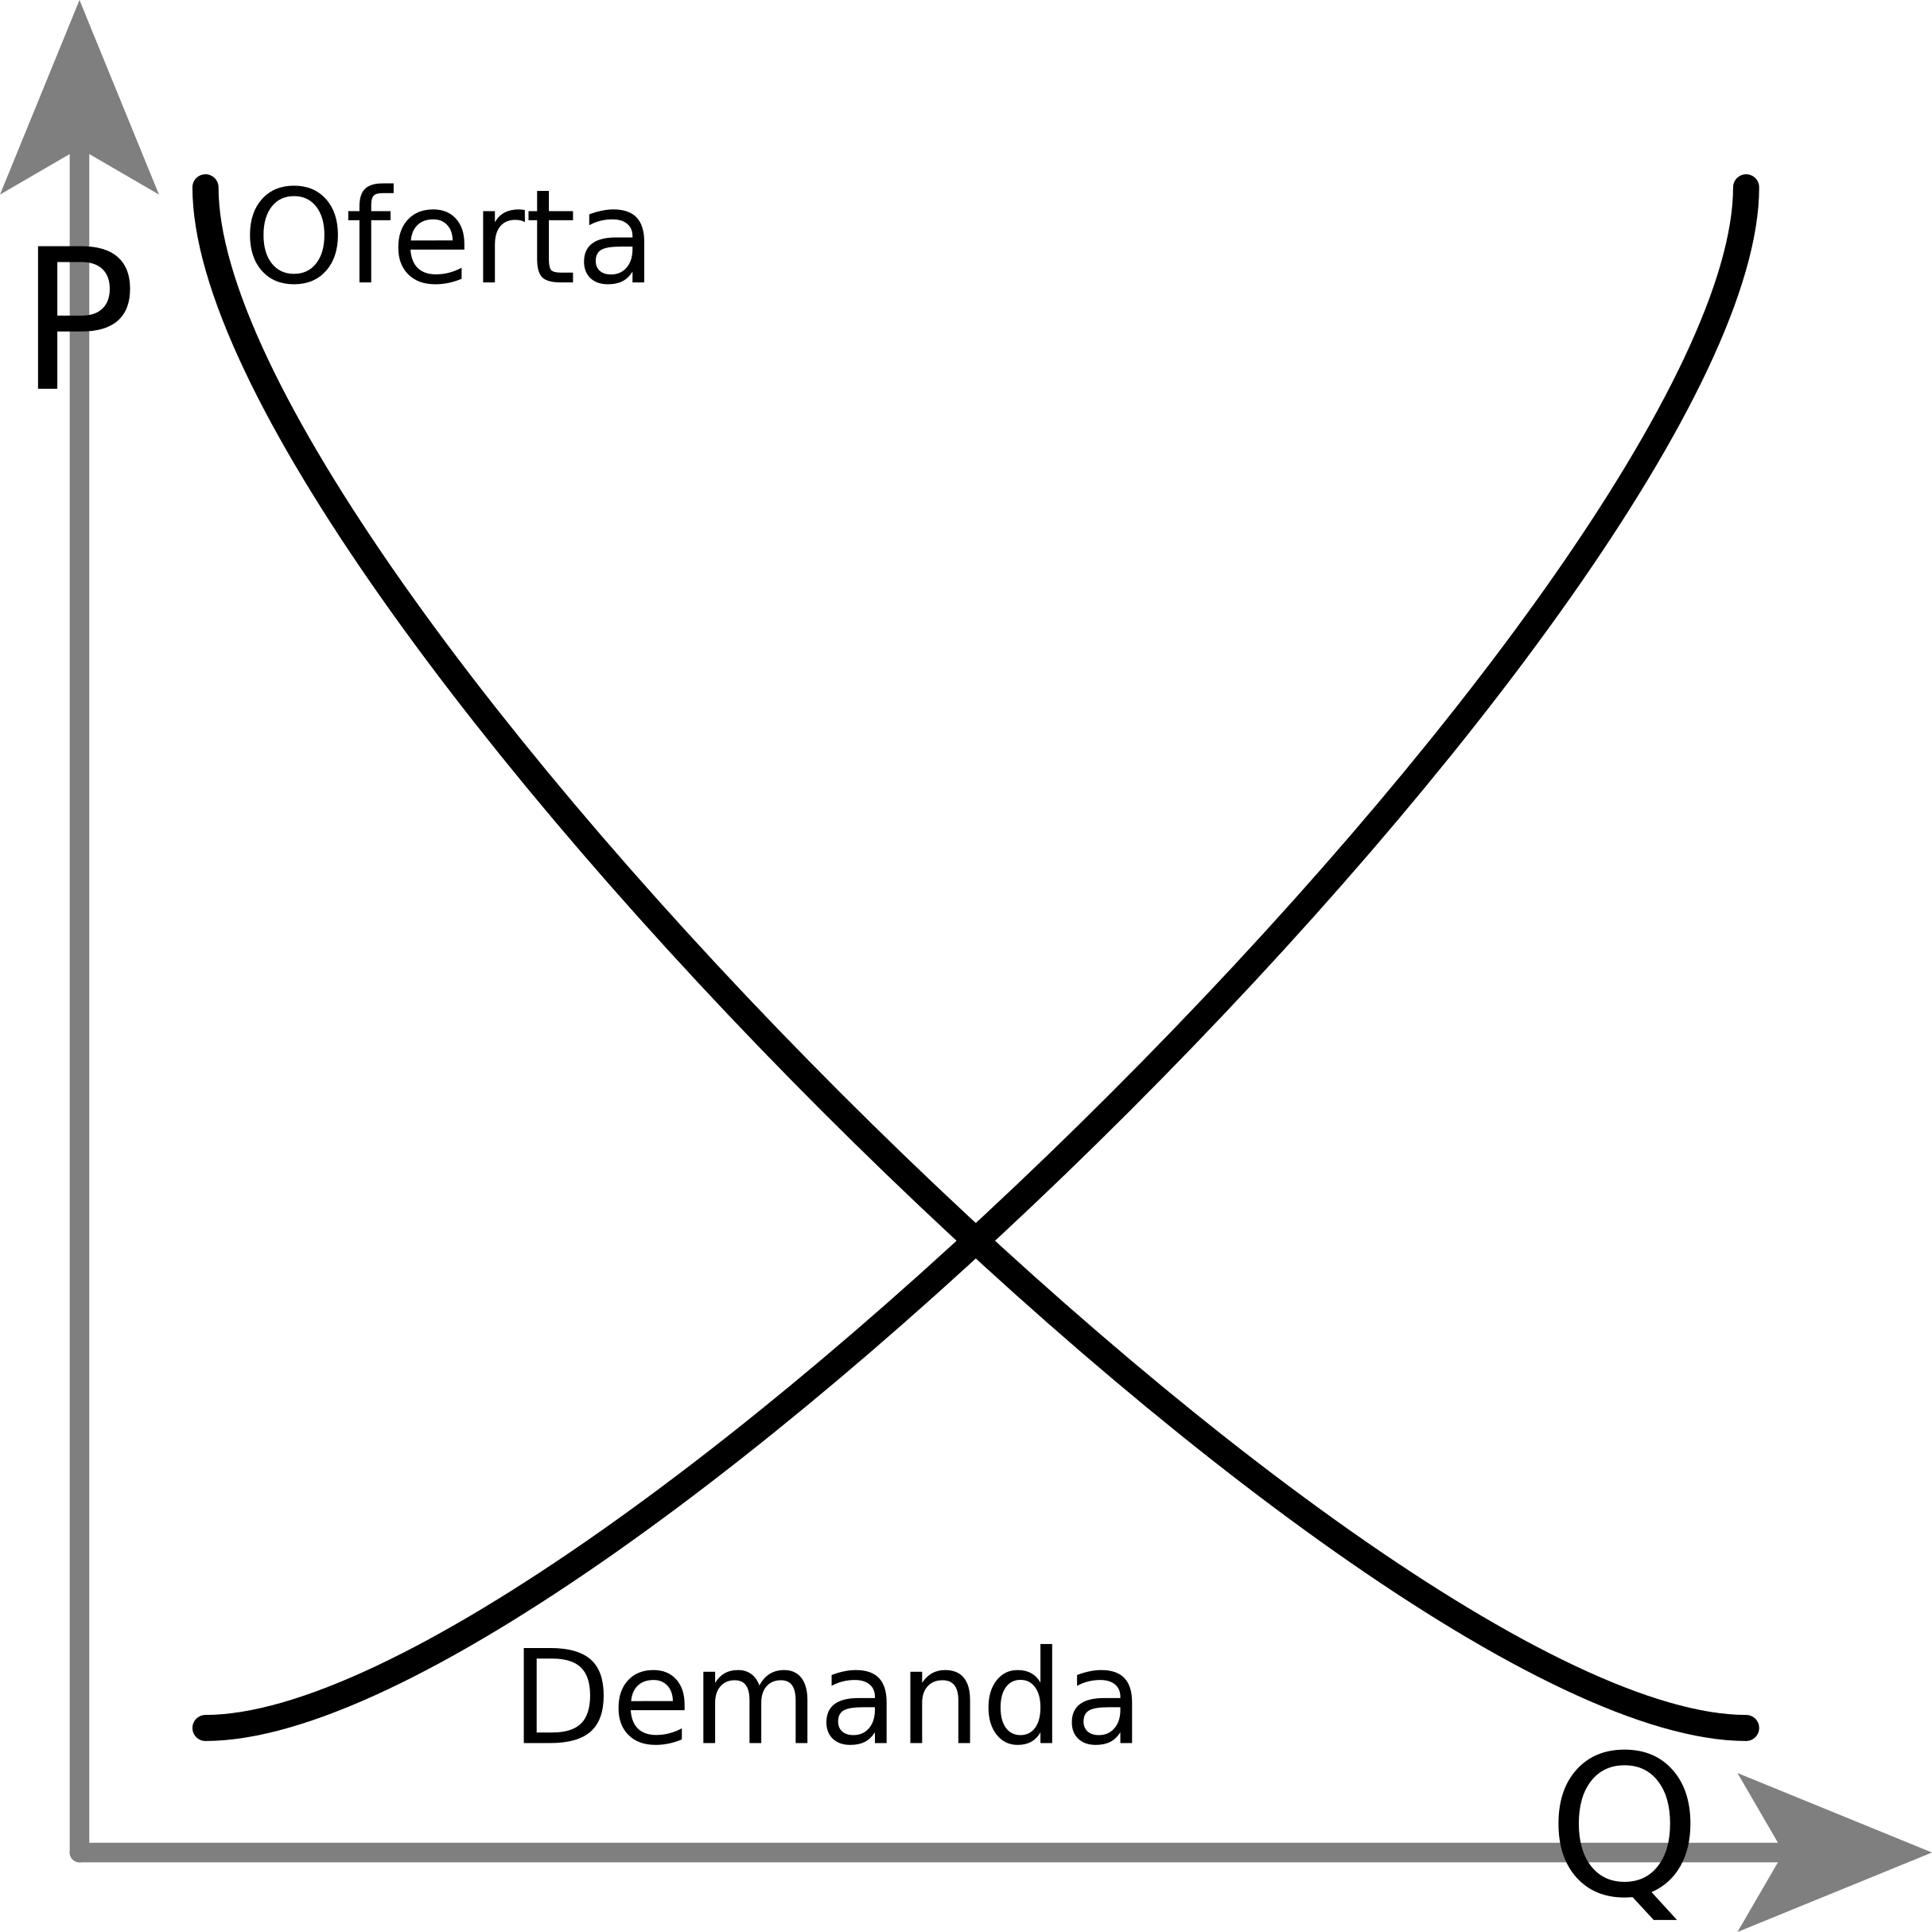
\includegraphics[width=0.5\textwidth]{img/leyofertademanda.png}
\end{center}

Why talking about "people's subjective preferences"? Because is with this law, being defined with the previous characteristics, that the \textit{desire} is based upon, and not for merely material issues. For example, if a person creates a "new drink" that contains: alcohol, bay leaves, rice starch, grenadine, soy sauce and tea, this will certainly be a "unique" drink; but if there isn't anyone who demands it (nobody to \textit{desire} it), this good, in terms of market, will not exist. If it's thought in terms of supply and demand by only looking the curve of quantity (a single existent drink) one could conclude that the price would have to be "really high"; but beyond the \textit{reference price}\footnote{This concept will be better explained at the end of this section, about the \textit{reference} price and the \textit{final} price.} that the creator assign to that good, if there is not any single person who is willing to buy such drink, then that good will be worth nothing in the market.

If the supply, in simple words, is "what someone offers" and the demand is "what someone wants", how can this be applied to money? Basically, those who demands money are people (or, to be extended in a wider category: the economic agents) of a territory in which it's used the money as a \textit{good of exchange}. Every person, within each country, uses money to exchange it for goods and services, for example, the argentinian peso, the chilean peso, the uruguayan peso, the guaraní, etcetera. The only supplier of money in the case of Argentina is the entity known as Central Bank.

What is a Central Bank? According to the authors Mochón and Beker:

\begin{quotation}
The Central Bank of the Argentine Republic is an autarchic entity\footnote{Meaning, a \textit{self-sufficient} entity.} and its capital is property of the State. It acts like a financial agent of the State. [...] It's related to the Executive Power through the Economy Ministry.

The primordial function of the Central Bank is to \textit{preserve the value of the currency}. \cite[p. 288]{mochobeker}
\end{quotation}

Next, it will be enumerated the different functions of the Central Bank \cite[pp. 288-289]{mochobeker}:

\begin{enumerate}
\item Guard and keep the gold reserves and currencies.
\item Being a financial agent of the national government.
\item Executing the monetary policies.
\item Being the bank of the banks.
\item Providing legal currency.
\item Being the superintendent of financial entities.
\item Executing exchange policies.
\end{enumerate}

Maybe the most foolish question would be, basing on the fifth point, why there could not be more than a money supplier? In other words, that there would be more than a single entity offering money (by fabricating and administrating it). In this case, no. Why? Because, precisely, the Central Bank is the only entity in charge of printing bills and minting coins that constitutes the money circulation of the country, in order to regulate and administrate it. Therefore, no private entity will legally have the power to print money, unless it's previously authorized to do that. And so, this will prevent any counterfeit money to be circulated in the country.

\subsection{Economic models}
Vaguely speaking, it has been mentioned the causes of inflation; nevertheless, it is needed to have a \textit{model} to methodologically analyze the economic phenomenons. According to the economists Zanotti, Krause and Ravier:

\begin{quotation}
A model is the result of the deduction [...]. It's about imaginary constructions in which it is abstracted some special characteristics and making hypothesis about the consequences of the absence of these conditions or the effects of its existence. \cite[p. 25]{elementos-econopol}
\end{quotation}

Models have to be consistent enough to explain a phenomenon in the most \textit{complete} possible way; but knowing that knowledge evolves through time; and the postulations are always subjected to revisions and refutations\footnote{By not allowing its revision, the knowledge would become \textit{dogmatic}, this means: the stipulated axioms cannot be questioned in any way, and any type of logical inconsistency or obsolescence it presents, must be equally accepted.}.

For example, one can stipulate a theory in which it is explained that water boils at one hundred Celsius. And the methodology behind its explanation, can support such data. However, if this experiment is repeated at 3.000 meters high, the water will boil at a temperature of ninety Celsius. Therefore, the main theory is discarded because of being \textit{insufficient} to explain such phenomenon, and its refuted with a new theory: the water boils at one hundred Celsius at sea level.

The authors mentions about the \textit{facts}:

\begin{quotation}
We're all very interested in the "facts", after all, we're all interested in learning economy in order to have a better interpretation of reality. The problem is, the facts itself don't say anything to us, unless we have a theory to interpret them. [...] Data has never given rise to any theory. \cite[p. 28]{elementos-econopol}
\end{quotation}

Following with the example: the phenomenon of boiling water by itself doesn't provide any kind of theory about it. If there is not anyone who wants to \textit{theorize} about, meaning, someone who offers an explanation in order to describe such phenomenon, the boiling water will pass unnoticed: it will only be a phenomenon.

How can it be collected such data? It could be used mathematics to offer a logic explanation; or it can be used the deduction to describe it. Here, we have two completely different methodologies to obtain the data:

\begin{quotation}
[...] Supporters of the empirical method were increasingly evolved towards the use of mathematics [...] while the supporters of the axiomatic-deductive method kept in the use of logical reasoning expressed in prose.

[...] No doubt that the use of the prose can lead to ambiguity, both due the different interpretation of the meaning of the words and the use of punctuation, but this is not necessarily solved by mathematics.

[...] Nevertheless, the economic laws are "qualitative", not "quantitative"; there are variables that cannot be susceptible of being quantified, among which the utility is one of them. The magnitude of the fall of a price by the increasing of its supply cannot be determined, and therefore mathematically expressed, because the subjective preferences cannot be measured. \cite[p. 26-27]{elementos-econopol}
\end{quotation}

The economic models, besides the description of phenomenons and offering justifications about it, they must also explain the interaction between people in such way that allows to demonstrate \textit{all} of them through the longest period of time possible in all the world. It cannot be created an economic theory that explains, only, a phenomenon in a very short period of time, under a few simple parameters, in a specific location; and pretend to be the leading model on the whole world economy (and even worse, making interventionists economic policies according to it).

About the time factor, the writer Henry Hazlitt say about this subject:

\begin{quotation}
There is a second main factor that spawns new economic fallacies every day. This is the persistent tendency of men to see only the immediate effects of a given policy, or its effects only on a special group, and to neglect to inquire what the long-run effects of that policy will be not only on that special group but on all groups. It is the fallacy of overlooking secondary consequences.

In this lies almost the whole difference between good economics and bad. The bad economist sees only what immediately strikes the eye; the good economist also looks beyond. The bad economist sees only the direct consequences of a proposed course; the good economist looks also at the longer and indirect consequences. The bad economist sees only what the effect of a given policy has been or will be on one particular group; the good economist inquires also what the effect of the policy will be on all groups. \cite[pp. 3-4]{hazlitt:econo1lec}
\end{quotation}

In lecture circles about libertarian economy, there is an analogy about this matter, and consist it with exemplifying it with a drug addict: the addict, at the moment of inhaling drugs, provokes an increasing amount of dopamine in his body (a neurotransmitter that helps to regulate emotions, motivations, and feelings of pleasure). The effect will surely be very pleasant in the short run; but, with time, this behavior tends to be in a drug-dependency, while the consequences in the long run will be: a weaker immune system, negative heart conditions, hepatic damage, brain damage, lung diseases, neurological degeneration and physical alteration of the body \cite{drug-problems}. Instead, if the addict stops consuming drugs, he will begin to suffer the drug withdrawal syndrome, whose most common symptoms are: anxiety, sweating, nausea, insomnia and hallucinations \cite{whitdrawal}; but in the long run, his body will no longer process any addictive substance, in which the damage to his body will be lesser.

This analogy serves as an explanation, about economic policies, to demonstrate that policies with a short-term benefit generally tends to unbalance the market and worsen the conditions in the long-term. The most beneficial policies in the long-term, however, tends to be "unpopular" in the short-term, without any kind of immediate benefit (even, it could seems to be harmful).

It can be done a comparison between economic policies and the analogy about drug addiction, with the next table:

\begin{center}
\begin{tabular}{|c|c|c|}
\hline 
\textbf{Order} & \textbf{Economic Policies} & \textbf{Drug addiction} \\ 
\hline 
1st & Inflationary problems & Withdrawal syndrome  \\ 
\hline 
2nd & Monetary "injection" & Drug use \\ 
\hline 
3rd & \multicolumn{2}{|c|}{Apparent solution of the problem} \\ 
\hline 
4th & Destruction of economy & Health deterioration \\ 
\hline 
\end{tabular} 
\end{center}

This cycle is repeated constantly until the country's economy can no longer resist anymore and falls into a hyperinflation, destroying the entire economy and plunging the country into an extreme poverty (such as the case of Venezuela). Analogously, the cycle of the addict repeats itself constantly until the body can no longer resist anymore and the person falls into a worse state of loss of consciousness (coma), plunging the body into a higher risk of death by organ damage due to the intoxication.

It is because of that the economic policies can \textit{never} be conceived as a series of beneficial policies in the short-term, but must have to be beneficial in the longest term possible (and this is not only applied to macroeconomic issues, but also to the personal finances) despite the apparent side effect in the short-term.

About the "universality" of economic theories, Ludwig von Mises writes about it:

\begin{quotation}
However, the situation is not quite the same with regard to economics as it is with mathematics and the natural sciences. Polylogism and irrationalism attack praxeology and economics. Although they formulate their statements in a general way to refer [...] it is the sciences of human action that they really have in view. They say that it is an illusion to believe that scientific research can achieve results valid for people of all eras, races, and social classes, and they take pleasure in disparaging certain physical and biological theories as bourgeois or Western. But if the soIution of practical problems requires the application of tbese stigmatized doctrines, they forget their criticism. The technology of Soviet Russia utilizes without scruple all the results of bourgeois physics, chemistry, and biology just as if they were valid for all classes. The Nazi engineers and physicians did not disdain to utilize the theories, discoveries, and inventions of people of "inferior" races and nations. The behavior of people of all races, nations, religions, linguistic groups, and social classes clearly proves that they do not endorse the doctrines of polylogism and irrationalism as far as logic, mathematics, and the natural sciences are concerned. \cite[pp. 5-6]{mises:lah}
\end{quotation}

About this quotation, there are several conceptions about economic theories throughout the world, with the justification that people, by being part of different cultures, their idiosyncrasy is different of others (even, some cultures can be incompatible with another). This implies that the \textit{action} of people will be different in every region of the world; and, therefore, it would be necessary to conceive the economic theory in another way. For example: an economic theory from Europe or from the United States of America would not function in a Latinamerican economy due to the different idiosyncrasy of the different regions; thus, it would be necessary to create a \textit{local} economic theory to explain local phenomenons.

This is a fallacy: the existence of differences in idiosyncrasies between two different cultures does not necessarily implies that the principles behind economic theories would be diametrically opposite from each other\footnote{This will be explained at the end of this section, mentioning the case of the explanation about "structural inflation" by the Latinamerican Developer School (Escuela Desarrollista Latinoamericana).}. Having cultural differences doesn't mean that, for example:

\begin{itemize}
\item When someone spends more than its income, that person have losses (no matter the justifications of its causes).
\item Saving money is the "sacrifice" of the immediate spending to be spent in the future (this leads to a financial \textit{discipline}: to abstain from the immediate benefits to be safe about the long-term benefits).
\item At a general level, when there is more than the same good in the market, one will be willing to pay less for the same good, because there will be a "wider" options to choose and therefore, will be "less valued" because of its abundance.
\item People will always find ways to be from a less state of satisfaction to a higher state of satisfaction (whether this is economic-related or not).
\end{itemize}

\begin{itemize}

For the naked eye, this would seems to be "simple" and obvious economic principles that have nothing to do with culture. Nevertheless, some economic theories, due to political issues (rather, \textit{ideological} issues) don't know or intentionally omit some of these points.

\subsection{Monetarists and Keynesian}
Within the discussions about monetary policies in Argentina, there is a debate about the nature of inflation. In one hand, there is the monetarist view, associated with the American economist Milton Friedman, who is linked with the so called Chicago School of Economy. On the other hand, there is the keynesian view, associated with the British economist John Maynard Keynes.

Keynes do a critique about classical liberal economist, like Adam Smith, with its monetary theory:

\begin{quotation}
So long as economists are concerned with what is called the Theory of Value, they have been accustomed to teach that prices are governed by the conditions of supply and demand [...]. But when they pass [...] to the Theory of Money and Prices, we hear no more of these homely but intelligible concepts where prices are governed by the quantity of money [...] and little or no attempt is made to relate these vague phrases to our former notions of the elasticities of supply and demand. If we reflect [...] it seems that the elasticity of supply must have become zero and demand proportional to the quantity of money; whilst in the more sophisticated we are lost in a haze where nothing is clear and everything is possible.

One of the objects of the foregoing chapters has been to escape from this double life and to bring the theory of prices [...] with the theory of value. The division of Economics between the Theory of Value and Distribution on the one hand and the Theory of Money on the other hand is, I think, a false division. \cite[pp. 292-293]{keynes}
\end{quotation}

For the Keynesian School, a rise of monetary supply does not generate inflation:

\begin{quotation}
In certain circumstances, in the very short-term, the demand of money can absorb the rise of the monetary supply without any alteration of prices. In this way, the relation between monetary supply and price levels are not so direct as what the monetarists hold, because an alteration of the quantity of money can have effects over the production. \cite[pág. 300]{mochobeker}
\end{quotation}

This means, for the keynesian vision, rising the monetary supply makes people who demands such money can "absorb" it in the very short-term, reducing the impact in the economy. This translates in the following example: it's done a "monetary stimulus" ("printing more money") in order to have more money circulating in the market. In a very short-term, this will be positive for the economy because the people in the country will demand such "monetary stimulus" and will utilize such money to spend it in whatever they desire. In this manner, money will not depreciate, due to the people's desire of having more money; and this will affect positively on the country's production because, now, these people can spend it in good and services that they could never been done if it wasn't for the stimulus.

On the other hand, Friedman is mainly known for his analysis on inflation, criticizing Keynes position. Here is shown eight of the ten main propositions considered the core of the monetarism \cite[pp. 36-37]{friedman:strike}:

\begin{enumerate}
\item There is a coherent relation, although not quite precise, between the growth rate of the quantity of money and the nominal income growth rate.
\item This relation is not evident at plain sight because the changes of monetary growth takes time to affect the income.
\item At average, a change in the monetary growth rate produces a change in the nominal growth rate between 6 and 9 months later [...].
\item The changes of the rate of nominal income growth normally it's reflected before in the production and almost nothing in the prices.
\item On average, the effects over prices comes between 6 and 9 months after the effect on the income and production, so the total delay [...] is roughly 12 to 18 months.
\item Even having in mind the delay on the monetary growth effect, the relation is far from being perfect. The changes in the short term are not "proportional".
\item In the short run, which it might be five or ten years, the monetary change affects primarily to the production. On the other hand, measuring by decades, the monetary growth rate affects primordially to prices.
\item From these propositions so far, it deducts that "inflation is always and everywhere a monetary phenomenon " in the sense that it is and can be produced only by a more rapid increase in the quantity of money than in the production.
\item The government spend can or can not be inflationary. It will be as long it's being financed by creating money, this means, minting coins or creating loan banks. 
\item The changes in the quantity of money affects to the interest rate in a direction at first, but later at the opposite direction. The faster monetary growth, at first, tends to lower the interest rate. But later, as the expenditure rises and stimulates the inflationary rise of prices, it also produces a rise on the demand of loans, which will tend to rise the interest rate. Therefore, this is the reason why at a worldwide level, the interest rate are lower in the countries where had a slower growth in the quantity of money. \cite[pp. 37-38]{friedman:paro}
\end{enumerate}

**************************

Incluso, autores actuales que se reconocen como neokeynesianos, como los antes mencionados Nicholas Gregory Mankiw u Olivier Blanchard, sí reconocen el fenómeno monetario de la inflación. Blanchard explica que:

\begin{quotation}
El crecimiento de la cantidad nominal de dinero solo afecta a la inflación.

[...] Aquí vemos que se obtiene un resultado similar de neutralidad en el caso de \textit{las variaciones de la tasa de crecimiento de la cantidad nominal de dinero}: las variaciones del crecimiento de la cantidad nominal de dinero no afectan a la producción ni al desempleo a medio plazo, sino que se traducen en una variación de la tasa de inflación de la misma cuantía.

Este último resultado también puede formularse diciendo que el único determinante de la inflación a medio plazo es el crecimiento de la cantidad nominal de dinero. Milton Friedman lo expresó de esa forma: \textit{la inflación es siempre y en todo lugar un fenómeno monetario}. Algunos factores, como el poder de monopolio de las empresas, el poder de los sindicatos, las huelgas, los déficit fiscales, el precio del petróleo, etc., no afectan a la inflación \textit{a medio plazo}, a menos que provoquen un aumento del crecimiento de la cantidad nominal de dinero. \cite[pág. 234]{blanchard}
\end{quotation}

**************************

On the other hand, Mankiw explains the \textit{quan-
tity theory of money}, given by the formula:

\begin{equation}\label{QTM}
M \times \overline{V} = P \times Y
\end{equation}

\begin{flushright}
\cite[p.~89]{mankiw:macroeconomics}
\end{flushright}

Where:

\begin{itemize}
\item $ M $ is the quantity of money.
\item $ \overline{V} $ the velocity of money, although it's assumed that the velocity is \textit{constant}.
\item $ P $ is the price of one unit of
output
\item $ Y $ is the total output of the economy.
\end{itemize}

Mankiw explains what happens when the Central Bank alters the monetary supply:

\begin{quotation}
First, the percentage change in the quantity of money \textit{M} is under the control of the central bank. Second, the percentage change in velocity \textit{V} reflects shifts in money demand; we have assumed that velocity is constant, so the percentage change in velocity is zero. Third, the percentage change in the price level \textit{P} is the rate of inflation; this is the variable in the equation that we would like to explain. Fourth, the percentage change in output \textit{Y} depends on growth in the factors of production and on technological progress, which for our present purposes we are taking as given. This analysis tells us that (except for a constant that depends on exogenous growth in output) the growth in the money supply determines the rate of inflation.

\textit{Thus, the quantity theory of money states that the central bank, which controls the money supply, has ultimate control over the rate of inflation. If the central bank keeps the money supply stable, the price level will be stable. If the central bank increases the money supply rapidly, the price level will rise rapidly.} \cite[p. 90]{mankiw}
\end{quotation}

\subsection{Criticism of the Monetarist School}
Beyond the critics done by the keynesians to the monetarist, there are several authors related to the Austrian School of Economics that also critics the "formal" and mathematical vision of the economy, just like a simple matter of calculus. The Spanish economist Jesús Huerta de Soto, in his book \textit{Money, Bank credit, and Economic cycles} criticizes Friedman's view:

\begin{quotation}
Monetarists not only overlook the role time and stages play in the economy’s productive structure. They also accept a mechanistic version of the quantity theory of money, a version they base on an equation which supposedly demonstrates the existence of a direct causal link between the total quantity of money in circulation, the "general level" of prices and total production.	

Supposing the "velocity of circulation" of money remains relatively constant over time, [...] monetarists believe [...] though in nominal terms the different factor incomes and production and consumption prices may increase by the same percentage as the money supply, in real terms they remain the same over time. [...] It is clear that the monetarist viewpoint is purely "macroeconomic" and ignores the microeconomic effects of monetary growth on the productive structure. [...] This approach stems from the lack of a capital theory which takes the time factor into account. \cite[pp. 522-523]{huertasoto:money}
\end{quotation}

The argentinian economist Martín Krause, on a commentary about the book \textit{Human Action}, demonstrates another critique of the quantity theory of money and its equation \eqref{QTM}:

\begin{quotation}
The error, in this sense, of a bad transcendence was the assumption of the money factor being neutral. Such idea induced many people to believe that the "level" of prices rises or lowers proportionally to the increment of decrement of the circulating quantity of money. It was forgotten that no variation recorded by money stocks can ever affect the prices of all goods and services at the same time and in the same proportion. 

[...] Instead of start by searching [...] the individual acts, it was pretended to study the subject by analizing the market economy as a whole. That forced to handle concepts such as the total quantity of existing money in the economy.

[...] Such discretion apparently made the price level doctrine acceptable. That way of thinking, however, merely suppose lucubrate in a typical vicious circle. The interchange equation, indeed, presupposes the same price level doctrine that pretends to prove. It's not more than a mathematical expression of that —unsustainable— thesis on which there's a uniform proportionality between prices and the quantitative variations of money.

By examining the interchange equation, it's presumed that one of its elements —the total quantity of money, the commercial volume, the circulating velocity— vary, without anyone asking which is the moving cause of such change. These mutations undoubtedly does not appear, in the economy, by spontaneous generation; what does actually change is the personal disposition of the individuals that acts in the correspondent economy, being the multiple acting of such persons what provokes the variations of what the price structure registers. Mathematical economists hide this effective demand and supply of money unleashed by each of every persons in the intervened economy. They recur, instead, on the misleading concept of the circulating velocity based on ideas taken by mechanics. \cite{krause:teomon}
\end{quotation}

\bibliographystyle{apacite}

\bibliography{biblio.bib}

\end{document}
